% Options for packages loaded elsewhere
\PassOptionsToPackage{unicode}{hyperref}
\PassOptionsToPackage{hyphens}{url}
\documentclass[
]{article}
\usepackage{xcolor}
\usepackage{amsmath,amssymb}
\setcounter{secnumdepth}{-\maxdimen} % remove section numbering
\usepackage{iftex}
\ifPDFTeX
  \usepackage[T1]{fontenc}
  \usepackage[utf8]{inputenc}
  \usepackage{textcomp} % provide euro and other symbols
\else % if luatex or xetex
  \usepackage{unicode-math} % this also loads fontspec
  \defaultfontfeatures{Scale=MatchLowercase}
  \defaultfontfeatures[\rmfamily]{Ligatures=TeX,Scale=1}
\fi
% lmodern мешает setmainfont (DejaVu) в XeLaTeX; кириллица без основного шрифта
% \usepackage{lmodern}
\ifPDFTeX\else
  % xetex/luatex font selection
  \setmainfont[]{DejaVu Serif}
  \setsansfont[]{DejaVu Sans}
  \setmonofont[]{DejaVu Sans Mono}
\fi
% Use upquote if available, for straight quotes in verbatim environments
\IfFileExists{upquote.sty}{\usepackage{upquote}}{}
\IfFileExists{microtype.sty}{% use microtype if available
  \usepackage[]{microtype}
  \UseMicrotypeSet[protrusion]{basicmath} % disable protrusion for tt fonts
}{}
\makeatletter
\@ifundefined{KOMAClassName}{% if non-KOMA class
  \IfFileExists{parskip.sty}{%
    \usepackage{parskip}
  }{% else
    \setlength{\parindent}{0pt}
    \setlength{\parskip}{6pt plus 2pt minus 1pt}}
}{% if KOMA class
  \KOMAoptions{parskip=half}}
\makeatother
\usepackage{longtable,booktabs,array}
\newcounter{none} % for unnumbered tables
\usepackage{multirow}
\usepackage{calc} % for calculating minipage widths
% Correct order of tables after \paragraph or \subparagraph
\usepackage{etoolbox}
\makeatletter
\patchcmd\longtable{\par}{\if@noskipsec\mbox{}\fi\par}{}{}
\makeatother
% Allow footnotes in longtable head/foot
\IfFileExists{footnotehyper.sty}{\usepackage{footnotehyper}}{\usepackage{footnote}}
\makesavenoteenv{longtable}
\usepackage{graphicx}
\makeatletter
\newsavebox\pandoc@box
\newcommand*\pandocbounded[1]{% scales image to fit in text height/width
  \sbox\pandoc@box{#1}%
  \Gscale@div\@tempa{\textheight}{\dimexpr\ht\pandoc@box+\dp\pandoc@box\relax}%
  \Gscale@div\@tempb{\linewidth}{\wd\pandoc@box}%
  \ifdim\@tempb\p@<\@tempa\p@\let\@tempa\@tempb\fi% select the smaller of both
  \ifdim\@tempa\p@<\p@\scalebox{\@tempa}{\usebox\pandoc@box}%
  \else\usebox{\pandoc@box}%
  \fi%
}
% Set default figure placement to htbp
\def\fps@figure{htbp}
\makeatother
\ifLuaTeX
  \usepackage{luacolor}
  \usepackage[soul]{lua-ul}
\else
  \usepackage{soul}
\fi
\setlength{\emergencystretch}{3em} % prevent overfull lines
\providecommand{\tightlist}{%
  \setlength{\itemsep}{0pt}\setlength{\parskip}{0pt}}
\usepackage{bookmark}
\IfFileExists{xurl.sty}{\usepackage{xurl}}{} % add URL line breaks if available
\urlstyle{same}
\hypersetup{
  hidelinks,
  pdfcreator={LaTeX via pandoc}}

\author{}
\date{}

\begin{document}

\textbf{МИНОБРНАУКИ РОССИИ\\
Федеральное государственное бюджетное образовательное\\
учреждение высшего образования\\
«Ярославский государственный университет им. П.Г. Демидова»\\
}Кафедра математического моделирования

\begin{quote}
Сдано на кафедру\\
«\_\_\_\_» \_\_\_\_\_\_\_\_\_\_\_\_\_\_2025 г.\\
Заведующий кафедрой\\
к. ф.-м. н., доцент\\
\_\_\_\_\_\_\_\_\_\_\_\_\_\_\_\_ И. С. Кащенко
\end{quote}

Курсовая работа

\textbf{Разработка концепции~физического генератора случайных чисел}

специальность 01.03.02 Прикладная математика и информатика

\begin{quote}
Научный руководитель\\
\ul{старший преподаватель}\_\_\\
\emph{(степень, звание)}\\
\ul{/ Д. А. Савинов}

\emph{(подпись) (ФИО)}

«\_\_\_» \_\_\_\_\_\_\_\_\_\_\_\_\_ 2025 г.

Студент группы \ul{ПМИ-31БО}

\ul{/ В. Д. Шестаков}

\emph{(подпись) (ФИО)}

«\_\_\_» \_\_\_\_\_\_\_\_\_\_\_\_\_ 2025 г.
\end{quote}

Ярославль 2025 г.

\textbf{СОДЕРЖАНИЕ}

ВВЕДЕНИЕ\ldots\ldots\ldots\ldots\ldots\ldots\ldots\ldots\ldots\ldots\ldots\ldots\ldots\ldots\ldots\ldots\ldots\ldots\ldots\ldots\ldots\ldots\ldots\ldots\ldots\ldots...
3

ГЛАВА 1. Теоретические основы генерации случайных
чисел\ldots\ldots\ldots\ldots\ldots.. 4

1.1. Основные понятия и
определения\ldots\ldots\ldots\ldots\ldots\ldots\ldots\ldots\ldots\ldots\ldots\ldots\ldots\ldots\ldots...
4

1.2. Классификация генераторов случайных
чисел\ldots\ldots\ldots\ldots\ldots\ldots\ldots\ldots\ldots\ldots.. 5

1.3. Методы оценки случайности
последовательностей\ldots\ldots\ldots\ldots\ldots\ldots\ldots\ldots.. 7

ГЛАВА 2. Анализ физических источников энтропии и их применение в
генераторах истинно случайных
последовательностей\ldots\ldots\ldots\ldots\ldots\ldots\ldots\ldots\ldots\ldots...
11

2.1. Электронные источники
шума\ldots\ldots\ldots\ldots\ldots\ldots\ldots\ldots\ldots\ldots\ldots\ldots\ldots\ldots\ldots\ldots\ldots.
11

2.2. Оптические и квантовые
источники\ldots\ldots\ldots\ldots\ldots\ldots\ldots\ldots\ldots\ldots\ldots\ldots\ldots\ldots\ldots{}
17

2.3. Механические и акустические
источники\ldots\ldots\ldots\ldots\ldots\ldots\ldots\ldots\ldots\ldots\ldots\ldots..
20

2.4.
Постобработка\ldots\ldots\ldots\ldots\ldots\ldots\ldots\ldots\ldots\ldots\ldots\ldots\ldots\ldots\ldots\ldots\ldots\ldots\ldots\ldots\ldots\ldots\ldots...
23

2.5. Уязвимости и
атаки\ldots\ldots\ldots\ldots\ldots\ldots\ldots\ldots\ldots\ldots\ldots\ldots\ldots\ldots\ldots\ldots\ldots\ldots\ldots\ldots\ldots...
25

ГЛАВА 3. Сравнительная характеристика и перспективы
применения\ldots\ldots. 28

3.1. Сравнительный анализ источников
энтропии\ldots\ldots\ldots\ldots\ldots\ldots\ldots\ldots\ldots\ldots\ldots{}
28

3.2. Перспективные направления развития
ФГСП\ldots\ldots\ldots\ldots\ldots\ldots\ldots\ldots\ldots\ldots\ldots{}
29

ЗАКЛЮЧЕНИЕ\ldots\ldots\ldots\ldots\ldots\ldots\ldots\ldots\ldots\ldots\ldots\ldots\ldots\ldots\ldots\ldots\ldots\ldots\ldots\ldots\ldots\ldots\ldots\ldots\ldots{}
31

СПИСОК ИСПОЛЬЗОВАННЫХ
ИСТОЧНИКОВ\ldots\ldots\ldots\ldots\ldots\ldots\ldots\ldots\ldots\ldots...
33

ПРИЛОЖЕНИЯ\ldots\ldots\ldots\ldots\ldots\ldots\ldots\ldots\ldots\ldots\ldots\ldots\ldots\ldots\ldots\ldots\ldots\ldots\ldots\ldots\ldots\ldots\ldots\ldots\ldots{}
35

Приложение 1 -- Статистические тесты пакета NIST
STS\ldots\ldots\ldots\ldots\ldots\ldots\ldots\ldots{} 35

Приложение 2 -- Сравнительная таблица характеристик источников
энтропии\ldots\ldots\ldots\ldots\ldots\ldots\ldots\ldots\ldots\ldots\ldots\ldots\ldots\ldots\ldots\ldots\ldots\ldots\ldots\ldots\ldots\ldots\ldots\ldots\ldots\ldots\ldots\ldots\ldots\ldots..
37

\textbf{ВВЕДЕНИЕ}

Случайные числа -- это одна из основ современных криптографических
систем, алгоритмов моделирования, шифрования и даже игровых механизмов.
Качество созданных последовательностей напрямую влияет на безопасность:
так, в 2012 году из-за недостатка энтропии в Android-устройствах,
злоумышленники смогли предсказать примерно 86\% закрытых ключей
Bitcoin-кошельков, сгенерированных на уязвимых гаджетах{[}1{]}. Подобные
инциденты доказывают, что генераторы псевдослучайных чисел (ГПСЧ),
используемые в программном обеспечении, уступают по надежности
аппаратным решениям на основе физических процессов.

Физические генераторы случайных чисел (ФГСЧ) получают энтропию из
недетерминированных явлений, например, таких как тепловые шумы
резисторов, лавинные пробои полупроводников, радиоактивный распад или
даже атмосферные помехи. В отличие от математических алгоритмов,
физические методы генерации СЧ вероятно менее уязвимы к обратному
инжинирингу, но их практическая реализация сталкивается со следующими
проблемами:

\begin{enumerate}
\def\labelenumi{\arabic{enumi}.}
\item
  Более низкая скорость работы;
\item
  Потенциально высокие временные и материальные затраты на
  конструирование, установку и настройку по сравнению с программными
  ГПСЧ;
\item
  Зависимость от среды (например, шумы микрофона могут исчезнуть в
  звукоизолированном помещении);
\item
  Аппаратные искажения (смещение распределения из-за неидеальности
  компонентов).
\end{enumerate}

Цель работы -- сравнить доступные источники энтропии (аудио-, радио-,
фотонные и механические шумы) для проектирования компактного ФГСЧ с
учетом:

\begin{enumerate}
\def\labelenumi{\arabic{enumi}.}
\item
  Критериев NIST STS (тесты на частоту, последовательности, энтропию);
\item
  Стоимости и простоты реализации;
\item
  Устойчивости к внешним воздействиям.
\end{enumerate}

Актуальность моего исследования связана с растущими требованиями к
безопасности в следующих областях:

\begin{enumerate}
\def\labelenumi{\arabic{enumi}.}
\item
  Криптографические системы (генерация ключей, seed-значений);
\item
  Защищенные микропроцессоры (TPM-модули, HSM);
\item
  Специализированные устройства (криптовалютные кошельки, банковские
  терминалы).
\end{enumerate}

Проблема уязвимостей в ГСЧ остается актуальной. Атака на чипы Infineon
TPM, получившая название «ROCA», показала, что даже корпоративные
решения могут содержать фатальные недостатки.

\textbf{ГЛАВА 1. Теоретические основы генерации случайных чисел}

\begin{enumerate}
\def\labelenumi{\arabic{enumi}.}
\item
  \textbf{Основные понятия и определения.}
\end{enumerate}

\textbf{Случайная последовательность} -- последовательность данных, в
которой отсутствуют статистические закономерности, а каждый следующий
элемент невозможно предсказать, зная предыдущие. С точки зрения
достоверности случайности последовательности разделяются на истинно
случайные и псевдослучайные.

\textbf{Истинно случайные последовательности (ИСП)} -- это
представленные в виде последовательности случайные числа. Случайные
числа являются реализацией некоторой случайной величины. Случайная
величина -- это функция над пространством элементарных событий,
принимающая вещественные значения с некоторыми вероятностями. Таким
образом, истинно случайные последовательности -- это последовательности
статистически независимых друг от друга величин, принимающих в
результате опыта одно из множества заранее непредсказуемых значений.
Связь между значениями случайной величины и соответствующими
вероятностями описывается законом распределения, который задается с
помощью функции распределения или связанной с ней функцией плотности
вероятности. Истинно случайные последовательности должны обладать
равномерным распределением.

Однако на практике далеко не всегда возможно непосредственно
использовать выходные данные источников истинно случайных чисел. Поэтому
обычно приходится использовать так называемые псевдослучайные
последовательности. \textbf{Псевдослучайная последовательность (ПСП)} --
это последовательность, состоящая из псевдослучайных двоичных чисел,
получаемых с помощью заданного детерминированного алгоритма, но
применяемых в качестве случайных. При этом обычно алгоритмы получения
ПСП используют специальное случайное начальное значение, или «зерно»
(seed). Для того чтобы ПСП могли использоваться в качестве случайных
последовательностей, они должны по статистическим свойствам быть близки
к ИСП.

\textbf{Энтропия} -- это мера хаотичности информации, неопределённости
или непредсказуемости. В контексте данной темы будет чаще встречаться
понятие источника энтропии, то есть источника, используемого для
получения случайной величины, которая необходима генераторам истинно
случайных последовательностей для формирования случайных чисел.

\textbf{Корреляция} -- это наличие связи между значениями выходной
последовательности, особенно показательна корелляция между соседними или
близкими по времени значениями. Другими словами, если два бита (или
числа), которые идут друг за другом, не полностью независимы друг от
друга, говорят, что между ними есть корреляция. Это плохо для ГСЧ,
поскольку идеальная случайная последовательность должна быть независимой
и равномерно распределённой -- т.е. каждый бит должен быть
непредсказуемым, независимо от предыдущих.

Коэффициент корреляции для удобства исследования случайных
последовтельностей может быть представлен в следующем виде{[}2{]}:

\[Corr(X_{t},X_{t + \tau}) = \frac{E\left\lbrack (X_{t} - \mu)(X_{t + \tau} - \mu) \right\rbrack}{\sigma^{2}}\]

где:

\begin{quote}
\(X_{t}\) --- значение на момент времени t,

τ --- сдвиг (лаг) по времени,

\emph{μ} --- математическое ожидание,

\(\sigma^{2}\) -- дисперсия.
\end{quote}

Если корреляция больше нуля при малых τ, это значит, что соседние
значения похожи --- и сигнал не полностью случаен.

\textbf{Спектральная плотность} (спектральная плотность мощности шума
или просто плотность шума) --- это количественная характеристика,
описывающая, как энергия случайного сигнала (в виде шума) распределена
по частотам. В контексте генераторов истинно случайных чисел,
спектральная плотность показывает, на каких частотах сосредоточена
энтропия, и является важным инструментом анализа качества и природы
случайности сигнала.

Спектральная плотность мощности случайного сигнала x(t) определяется
как{[}2{]}:

\[S_{x}(f) = {\lim_{T \rightarrow \infty}{\frac{1}{T}\left| \int_{\frac{- T}{2}}^{\frac{T}{2}}{x(t)e^{2\pi ift}}dt \right|}}^{2}\]

В контексте источников энтропии, плоский (частотно-независимый) спектр
\emph{S(f) = const} соответствует белому шуму --- идеальному случаю,
когда энтропия равномерно распределена по частотам.

\begin{enumerate}
\def\labelenumi{\arabic{enumi}.}
\setcounter{enumi}{1}
\item
  \textbf{Классификация генераторов случайных чисел.}
\end{enumerate}

Генераторы случайных чисел разделяются на две основные категории:
истинные генераторы случайных чисел (ГИСП) и псевдослучайные генераторы
чисел (ГПСП). ГИСП создают случайные числа, опираясь на физические
источники, к примеру, шум от тепловых, атмосферных или радиоактивных
явлений. С другой стороны, ГПСП генерируют числа детерминированно на
основе начального значения, которое должно быть трудно предсказуемым и
безопасным. Если кто-либо извне получает доступ к нему или может влиять
на его генерацию, то он может предсказать вывод ГПСП, что будет являться
нарушением безопасности. Схема общей структуры модуля ГИСП представлена
на рисунке 1{[}9{]}{[}12{]}.

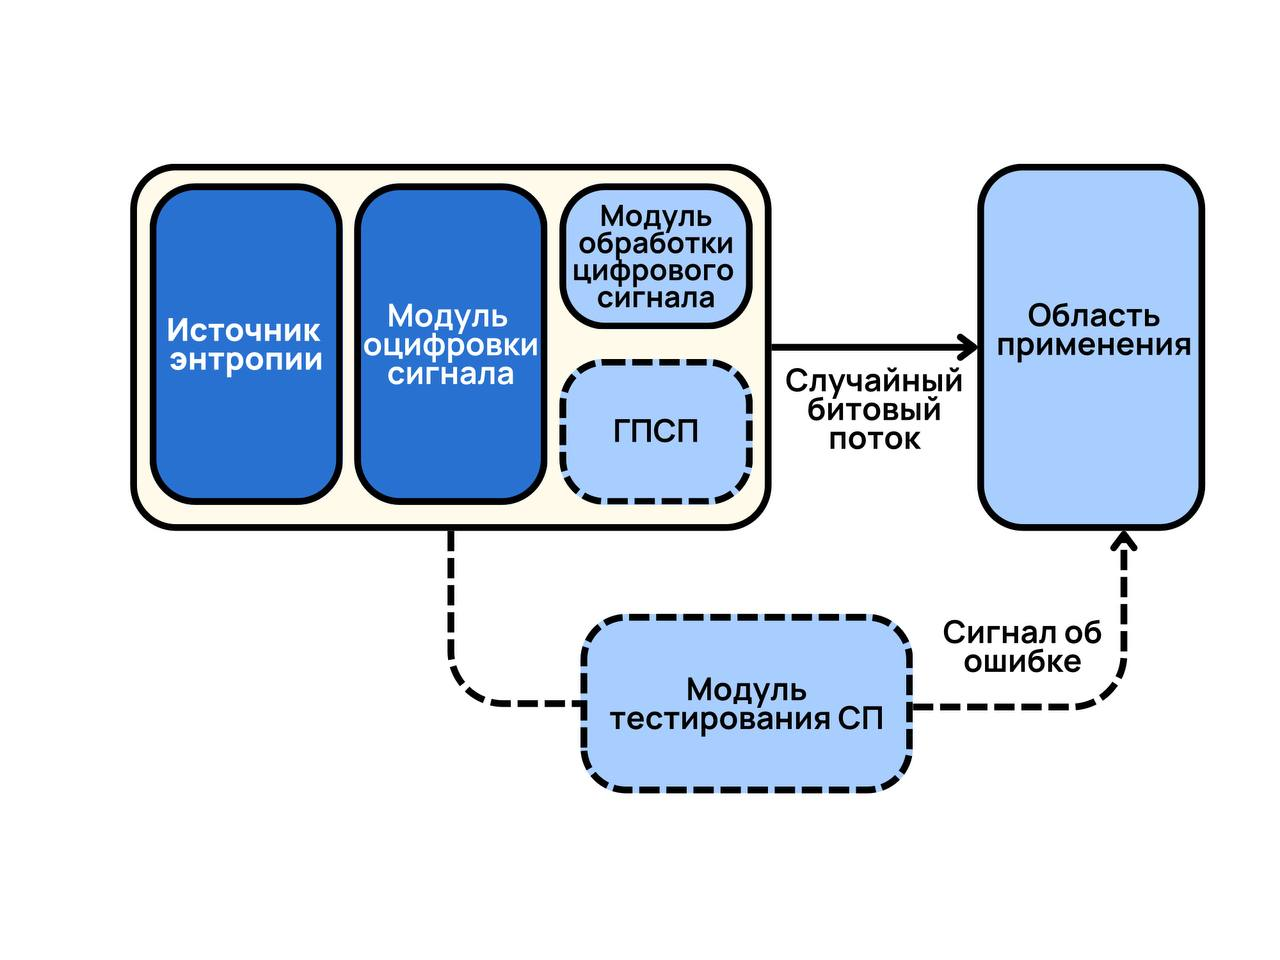
\includegraphics[width=4.68611in,height=2.89514in]{pandoc_media/media/image1.png}Рисунок
1

Генератор псевдослучайных последовательностей (ГПСП) -- это функция,
которая принимает короткое случайное начальное значение и выдает более
длинную последовательность бит, которая кажется случайной.
Криптографически стойкий генератор псевдослучайных чисел (КСГПСП)
обладает свойствами стойкости к криптоанализу и является важным
средством в обеспечении безопасности криптографических систем, таких как
шифрование данных, создание ключей и другие приложения, где требуется
случайность с высоким уровнем безопасности. Для обеспечения
криптографической безопасности вывод ГПСП должен быть вычислительно
неотличим от случайной строки. Это означает, что при наличии короткого
префикса последовательности должно быть вычислительно невозможно
предсказать оставшуюся часть последовательности без знания начального
значения.

Кроме этого, возможно выделить гибридный тип генератора случайных чисел,
который совмещает в себе ГИСП, для формирования начального значения
(seed), и ГПСП, который использует полученное начальное значение для
дальнейших генераций, что позволяет такому классу ГСП поддерживать
достаточно высокий уровень криптографической безопасности и скорости
генерации.

Также ГСП можно классифицировать по методам генерации случайных
последовательностей{[}4{]}:

Табличные генераторы. Используют уже готовые таблицы, из которых
получают случайные последовательности. Их главное преимущество
заключается в высокой скорости работы, а недостаток в большом объёме
хранимых данных для достаточной безопасности сформированной
последовательности.

Алгоритмические генераторы. Подобные генераторы используют определенные
математические формулы для создания последовательностей случайных чисел.
Конечно, они могут генерировать исключительно псевдослучайные
последовательности. Их реализация при приближении к истинно случайным
величинам требует значительных вычислительных ресурсов компьютера.

Физические генераторы. ГСП данного типа используют внешние явления и
воздействия в качестве источника случайных величин, опираясь на
показания датчиков или индикаторов, фиксирующих какой-либо случайный
физический процесс, либо получая информацию о естественно происходящем
или искусственно вызванном хаотическом явлении иными способами.
Простейшими примерами физического генератора случайных
последовательностей могут служить монета (игра в «орла» и «решку») либо
игральные кости. О других наиболее практико-применимых источниках
энтропии для физических ГСП будет сказано позже.

\begin{enumerate}
\def\labelenumi{\arabic{enumi}.}
\setcounter{enumi}{2}
\item
  \textbf{Методы оценки случайности последовательностей}
\end{enumerate}

Случайные последовательности, созданные как физическими, так и
алгоритмическими генераторами в особенности требуют оценки качества их
действительной случайности. Существует несколько способов тестирования
случайных последовательностей:

Графические тесты. Свойства последовательностей отображаются в виде
графических зависимостей, по виду которых делают выводы о свойствах
исследуемой последовательности. К данной категории можно отнести
следующие тесты: гистограмма распределения элементов последовательности,
распределение на плоскости, проверка на монотонность и т.д. На рисунке 2
представлен пример графического теста «распределение на плоскости».
Слева результат тестирования отрицательный, справа --
положительный{[}10{]}.

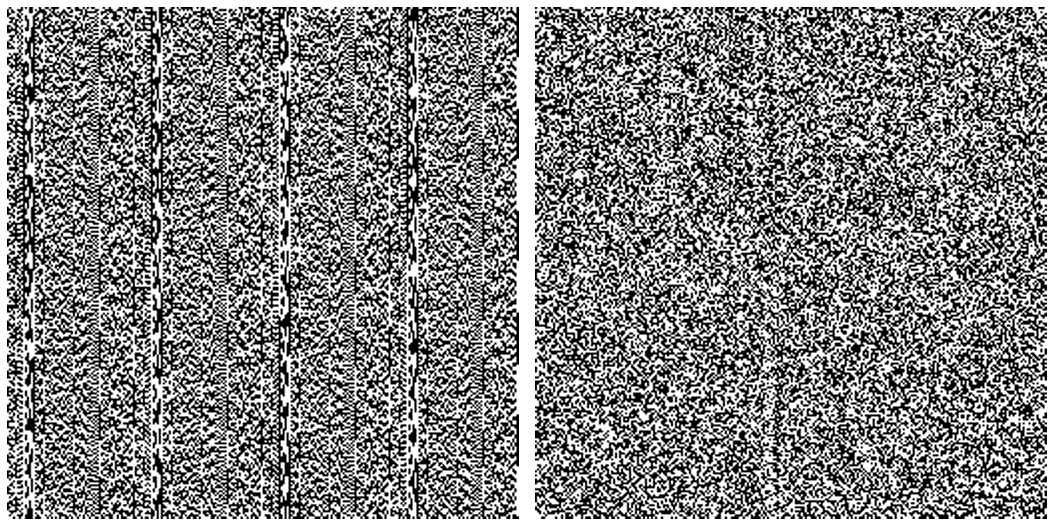
\includegraphics[width=5.10417in,height=2.53958in]{pandoc_media/media/image2.png}

Рисунок 2.

Статистические тесты. Основным критерием, применяемым для анализа
качества генераторов случайных чисел, являются статистические тесты. Они
проверяют соответствие последовательностей математическим свойствам
случайных данных. В основе тестов лежит понятие нулевой гипотезы. За
нулевую гипотезу принимается предположение, что последовательность
является истинно случайной. Следовательно, если нулевая гипотеза верна,
то наш генератор производит достаточно хорошие случайные числа.
Существует 4 варианта возможных выводов по результатам тестов{[}3{]}:

\begin{enumerate}
\def\labelenumi{\arabic{enumi}.}
\item
  Сделан вывод о том, что последовательность случайна, и это верный
  вывод
\item
  Сделан вывод о том, что последовательность не случайна, хотя она была
  на самом деле случайна. Такие ошибки называют ошибками первого рода
\item
  Последовательность признана случайной, хотя на самом деле таковой не
  является. Такие ошибки называют ошибками второго рода
\item
  Последовательность справедливо отбракована
\end{enumerate}

Наиболее популярные пакеты статистических тестов случайных и
псевдослучайных последовательностей {[}6{]} представлены в таблице 1.

Таблица 1.

{\def\LTcaptype{none} % do not increment counter
\begin{longtable}[]{@{}
  >{\raggedright\arraybackslash}p{(\linewidth - 6\tabcolsep) * \real{0.0520}}
  >{\raggedright\arraybackslash}p{(\linewidth - 6\tabcolsep) * \real{0.1909}}
  >{\raggedright\arraybackslash}p{(\linewidth - 6\tabcolsep) * \real{0.3721}}
  >{\raggedright\arraybackslash}p{(\linewidth - 6\tabcolsep) * \real{0.3757}}@{}}
\toprule\noalign{}
\begin{minipage}[b]{\linewidth}\raggedright
№
\end{minipage} & \begin{minipage}[b]{\linewidth}\raggedright
Пакеты статистических тестов
\end{minipage} & \begin{minipage}[b]{\linewidth}\raggedright
Тестирование СП длины до 300 бит
\end{minipage} & \begin{minipage}[b]{\linewidth}\raggedright
Тестирование СП длины порядка 10⁶ бит
\end{minipage} \\
\midrule\noalign{}
\endhead
\bottomrule\noalign{}
\endlastfoot
1 & Тесты Д. Кнута & -- & \begin{minipage}[t]{\linewidth}\raggedright
• критерий частот\\
• критерий серий\\
• критерий «максимум-t»\\
• критерий монотонности\strut
\end{minipage} \\
2 & NIST STS & \begin{minipage}[t]{\linewidth}\raggedright
• частотный побитовый тест (Frequency Test)\\
• частотный блочный тест (Frequency Test within a Block)\\
• тест на последовательность одинаковых бит (Runs Test)\\
• тест на совпадение неперекрывающихся шаблонов (Non-overlapping
Template Matching Test)\\
• тест на периодичность (Serial Test)\\
• тест рангов бинарных матриц (Binary Matrix Rank Test)\\
• тест приблизительной энтропии (Approximate Entropy Test)\\
• тест кумулятивных сумм (Cumulative Sums (Cusum) Test)\\
• тест на самую длинную последовательность «1» в блоке (Test for the
Longest Run of Ones in a Block)\strut
\end{minipage} & \begin{minipage}[t]{\linewidth}\raggedright
• частотный блочный тест (Frequency Test within a Block)\\
• тест на последовательность одинаковых бит (Runs Test)\\
• тест на совпадение перекрывающихся шаблонов (Overlapping Template
Matching Test)\\
• тест на периодичность (Serial Test)\\
• тест на линейную сложность (Linear Complexity Test)\\
• спектральный тест (Discrete Fourier Transform Test)\\
• универсальный статистический тест Маурера (Maurer Universal Test)\\
• тест рангов бинарных матриц (Binary Matrix Rank Test)\\
• тест приблизительной энтропии (Approximate Entropy Test)\\
• тест на произвольные проходы (Random Excursions Test)\\
• другой тест произвольные проходы (Random Excursions Variant Test)\\
• тест на самую длинную последовательность «1» в блоке (Test for the
Longest Run of Ones in a Block)\strut
\end{minipage} \\
3 & DIEHARD & -- & • проверка промежутков между днями рождений (The
Birthday Spacing Test) \\
4 & TestU01 & \begin{minipage}[t]{\linewidth}\raggedright
• тест веса Хэмминга (Hamming Weight Test)\\
• тест автокорреляции (Autocorrelation)\\
• тест случайных проходов (Random Walk Test)\\
• тест на самую длинную последовательность «1» в блоке (Longest Run of
1\textquotesingle s Test)\strut
\end{minipage} & \begin{minipage}[t]{\linewidth}\raggedright
• тест веса Хэмминга (Hamming Weight Test)\\
• тест серий и разрывов (Run and Gap Test)\\
• тест сложности последовательности на основе алгоритма Лемпела-Зива
(Lempel-Ziv Complexity Test)\\
• тест автокорреляции (Autocorrelations Test)\\
• тест на самую длинную последовательность «1» в блоке (Longest Run of
1\textquotesingle s Test)\\
• CAT тест (CAT Test)\strut
\end{minipage} \\
5 & Crypt-XS & \begin{minipage}[t]{\linewidth}\raggedright
• тест частот (Frequency Test)\\
• тест бинарной производной (Binary Derivative Test)\strut
\end{minipage} & • тест сложности последовательности (Complexity
Test) \\
\end{longtable}
}

Наиболее подходящими тестами для оценки СП в выбранной теме будут NIST
STS (Statistical Test Suite), так как они в совокупности обладают
достаточной строгостью и полнотой оценки, имеют свой стандарт NIST SP
(Special Publication) 800-22, который является достаточно известным в
сфере криптографии и наиболее часто применяются для оценки именно
физических ГСП{[}8{]}. Для общего ознакомления каждый из статистических
тестов пакета NIST STS с кратким описанием приведены в виде таблицы в
приложении 1.

Для физических ГСП особенно важны спектральный тест (№12) и тест Маурера
(№13){[}5{]}. Спектральный тест анализирует последовательность в
частотной области с помощью преобразования Фурье, чтобы обнаружить
скрытые периодичности или аномальные пики. Подобный тест способен
выявить периодические паттерны, которые могут появляться в физическом
ГСП по нескольким причинам, таким как колебания напряжения в схеме,
влияние внешних электромагнитных помех и дефекты датчиков (например,
шумового диода). Спектральный тест обнаруживает такие скрытые частотные
компоненты, которые не видны в статистических тестах на битовом уровне.

Тест Маурера оценивает алгоритмическую сложность последовательности,
проверяя, насколько она «несжимаема». Случайные данные не должны
допускать оптимизации при сжатии. Он особенно важен для проверки
физических генераторов потому, что физические процессы (например, шум в
транзисторах) иногда порождают статистически случайные, но
алгоритмически простые последовательности. Тест Маурера способен выявить
такие случаи. Кроме этого, генераторы с низкой энтропией (например,
из-за «залипания» датчика в определённых состояниях) проваливают этот
тест.

Дополнительное подтверждение необходимости тестирования физических
генераторов тестами 12 и 13 вытекает из того, что стандарт NIST SP
800-22 рекомендует эти тесты для аппаратных генераторов, используемых в
криптографии. Практический пример: квантовые ГСП обязательно проверяют
спектральным тестом на предмет квантовых корреляций.

\textbf{\hfill\break
}

\textbf{ГЛАВА 2. Анализ физических источников энтропии и их применение в
генераторах истинно случайных последовательностей.}

\textbf{2.1. Электронные источники шума.}

При проектировании интегральных схем шум неизбежен и нежелателен. Однако
в физических ГИСП улавливание и усиление непредсказуемых и
неконтролируемых человеком источников шума являются основополагающими
принципами. Для хорошей модели источника энтропии сам источник должен
представлять собой белый шум с гауссовым распределением. Таким образом,
качество источника энтропии напрямую зависит от наблюдаемых свойств
генерируемого им шума.

Выделим и проанализируем 4 основных вида электронных источников энтропии
пригодных для разработки ГСП:

\begin{enumerate}
\def\labelenumi{\arabic{enumi}.}
\item
  Тепловой шум
\item
  Дробовой шум
\item
  Лавинный шум
\item
  Мерцающий шум
\end{enumerate}

\textbf{Тепловой шум}, также называемый шумом Джонсона-Найквиста или
термическим шумом -- это электронный шум, возникающий в результате
теплового возбуждения носителей заряда, обычно электронов, в
электрическом проводнике. Этот вид шума возникает в любом резисторе с
ненулевой температурой и имеет строго физическую природу, основанную на
хаотичном тепловом движении электронов. Белый гауссов шум, генерируемый
резистором за счёт тепловой агитации носителей заряда впервые был описан
в работах Джона Б. Джонсона и Гарри Найквиста в 1928 году.

Среднеквадратичное напряжение теплового шума в заданной полосе (согласно
формуле Найквиста){[}11{]}{[}13{]}:

\[\overline{e_{t}^{2}} = 4kTR\mathrm{\Delta}f\]

где:

\begin{quote}
\(\overline{e_{t}^{2}}\) -- cреднеквадратичное напряжение шума,

\emph{k} ≈ 1.38×10\textsuperscript{23} Дж/К~-- постоянная Больцмана,

\emph{T} -- абсолютная температура резистора в кельвинах,

\emph{R} -- сопротивление в омах,

\(\mathrm{\Delta}f\) = \emph{f\textsubscript{upper}} --
\emph{f\textsubscript{lower }}-- выбранная для измерения полоса частот
\end{quote}

Спектральная плотность напряжения такого шума задаётся формулой{[}11{]}:

\[S_{f} = 4kTR\frac{hf}{kT}(exp{\frac{hf}{kT} - 1)}^{- 1}\]

где:

\begin{quote}
\emph{h} ≈ 6,626×10\textsuperscript{−34}~Дж*с \emph{--} постоянная
Планка

\(S_{f}\) -- спектральная плотность (В\textsuperscript{2}*с)
\end{quote}

График зависимости спектральной плотности от частоты при комнатной
температуре представлен на рисунке 3.

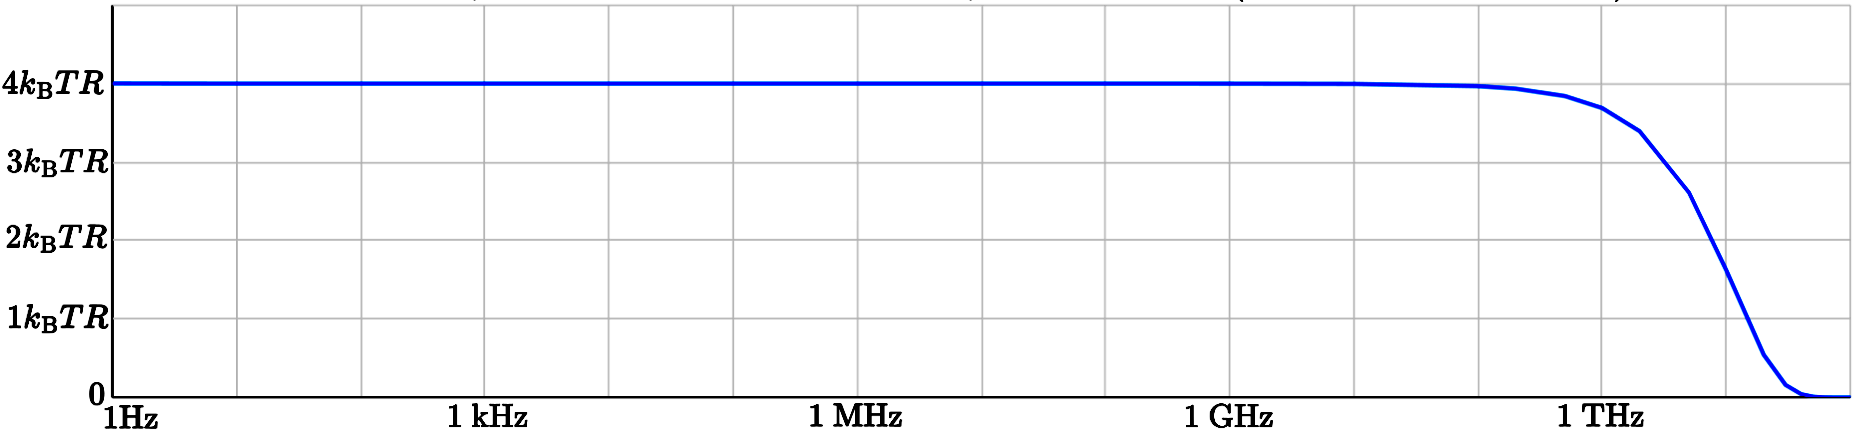
\includegraphics[width=6.49653in,height=1.51597in]{pandoc_media/media/image3.png}
Рисунок 3.

Для области соответствующей условию:

\[\frac{hf}{kT} \ll 1\]

Иными словами, для частот, значительно меньших, чем

\[f_{\max} \approx \frac{kT}{h}\]

\[(f_{\max} \approx 6 \times 10^{12}Гц\ при\ 300К)\]

Можем считать спектральную плотность постоянной независимой от
частоты{[}11{]}:

\[S_{f} = \frac{\overline{e_{t}^{2}}}{\mathrm{\Delta}f} = 4kTR\]

Эта спектральная плотность не зависит от частоты (в диапазоне до
десятков гигагерц), поэтому шум считается белым.

Чтобы использовать этот шум в ГИСП, необходимо выполнить несколько
этапов:

1. Формирование сигнала. Электрическое напряжение, наведённое тепловым
шумом на резисторе, усиливается с помощью малошумящего операционного
усилителя.

2. Ограничение полосы частот. Сигнал пропускается через полосовой
(bandpass) фильтр, чтобы исключить внешние помехи и отсечь побочные
частоты.

3. Оцифровка. Полученный аналоговый сигнал дискретизируется и квантуется
с помощью АЦП (аналогово-цифрового преобразователя). Результатом
является последовательность значений, например 8- или 12-битных.

4. Преобразование в случайные биты. Используется постобработка:
вырезание младших битов, хэш-функции или экстракция с помощью
алгоритмов, таких как Von Neumann extractor или Hash-based extractor,
чтобы устранить корреляции и повысить энтропию.

Количество энтропии, генерируемое за единицу времени, зависит от ширины
полосы Δ\emph{f}, температуры \emph{T}, сопротивления \emph{R}, точности
АЦП и скорости дискретизации. Важно понимать, что после АЦП не все биты
одинаково случайны: старшие биты могут быть предсказуемы, особенно при
низком уровне шума. Поэтому чаще всего используются младшие биты, иногда
с дополнительной энтропийной компрессией.

Преимущества использования теплового шума в роли источника энтропии в
ГИСП:

\begin{itemize}
\item
  Высокая надёжность и физическая непредсказуемость.
\item
  Отсутствие квантовых эффектов (при правильно настроенном полосовом
  фильтре).
\end{itemize}

Недостатки:

\begin{itemize}
\item
  Уязвимость к внешним электромагнитным помехам.
\item
  Необходимость сложной постобработки для получения равномерного
  распределения.
\item
  Необходимость температурной стабилизации для поддержания стабильного
  уровня шума.
\end{itemize}

Блок-схема проектирования ГИСП на основе теплового шума может выглядеть
следующим образом (рисунок 4):

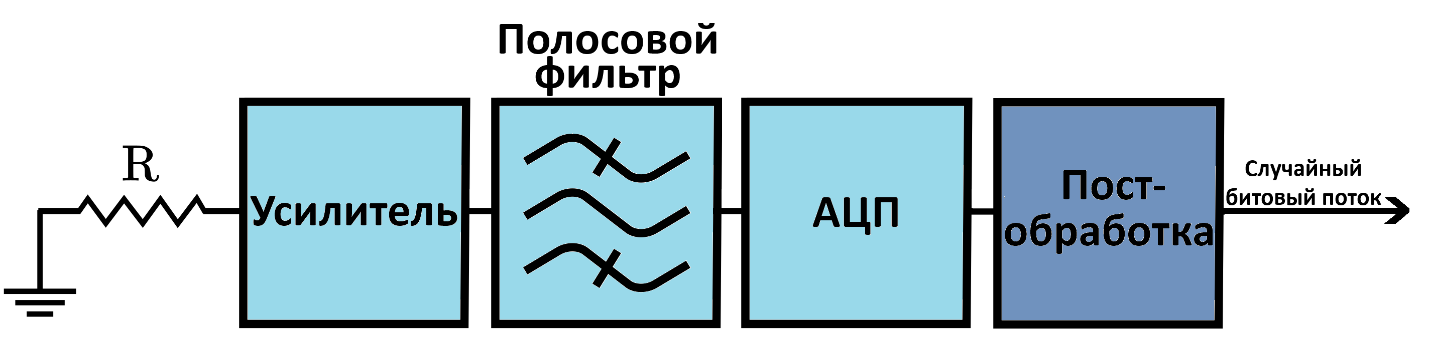
\includegraphics[width=6.49583in,height=1.55625in]{pandoc_media/media/image4.png}

Рисунок 4

Изучая в 1918 году тепловой шум с использованием теорий Эйнштейна,
Уолтер Шоттки экспериментально обнаружил другой вид шума -- дробовой
шум.

\textbf{Дробовой шум} (shot noise\emph{,} шум Пуассона) -- это
электронный шум, связанный с дискретной (квантованной) природой
электрического тока. Он возникает из-за того, что заряд переносится не
непрерывно, а в виде отдельных частиц -- электронов. Когда электроны
пересекают потенциальный барьер (например, в p-n переходе, вакуумном
диоде, туннельном переходе и т.д.), они делают это случайным образом,
независимо друг от друга, что приводит к флуктуациям тока, даже если
средний ток постоянен. Термин «дробовой шум» (а также дробовой эффект)
возник в связи с тем, что благодаря ему в громкоговорителе, подключённом
к выходу усилителя или радиоприёмника, появляется акустический шум,
воспринимаемый ухом как напоминающий шум сыплющихся дробинок.

Впервые дробовой шум был теоретически описан Уолтером Шоттки в 1918
году, когда он исследовал шумовые характеристики вакуумных ламп.

Среднеквадратичное значение тока шума Шоттки за интервал времени
определяется как{[}12{]}{[}13{]}:

\[\overline{i_{s}^{2}} = 2qI\Delta f\]

где:

\begin{quote}
\(\overline{i_{s}^{2}}\)\hspace{0pt}\hspace{0pt} -- дисперсия тока шума,

\emph{q} ≈ 1.6×10\textsuperscript{−19} Кл --- заряд электрона,

\emph{I} -- средний ток (А),

Δ\emph{f} -- ширина полосы частот (Гц).
\end{quote}

Спектральная плотность дробового шума также постоянна во всём частотном
диапазоне и задаётся формулой{[}11{]}:

\[S_{I}(f) = 2qI\]

В отличие от теплового шума, который зависит от температуры, дробовой
шум не зависит от температуры, но зависит от среднего тока I.

Дробовой шум наблюдается только в условиях, когда поток зарядов не
является непрерывным:

\begin{itemize}
\item
  в вакуумных диодах,
\item
  в фотоэлектронных приборах,
\item
  в туннельных диодах,
\item
  в слабонасыщенных p-n переходах,
\item
  в фотодетекторах (где ток создаётся фотонами, а не внешним
  напряжением).
\end{itemize}

В металлических проводниках дробовой шум обычно подавлен за счёт эффекта
выравнивания потенциала и действия Паули, поэтому там преобладает
тепловой шум.

Чтобы использовать дробовой шум в генераторах истинных случайных чисел,
реализуется следующая схема:

1. Формирование тока. Используется p-n переход или фотодиод в режиме
слаботекущего тока (порядка наноампер --- микроампер). При этом
создаётся ток, насыщенный дробовым шумом.

2. Преобразование в напряжение. Ток преобразуется в напряжение с помощью
токозависимого усилителя или прецизионного резистора.

3. Усиление. Сигнал усиливается, при этом важно сохранить соотношение
сигнал/шум и не вносить дополнительный шум от усилителя.

4. Ограничение полосы частот. Подача на полосовой фильтр для выделения
нужного частотного диапазона.

5. Оцифровка. Сигнал поступает на АЦП. Аналогично тепловому шуму,
оцифрованный сигнал содержит "сырые" данные.

6. Постобработка. Применяются алгоритмы, повышающие качество случайных
битов --- например, хэширование или алгоритм фон Неймана.

Как и тепловой шум, дробовой шум имеет равномерную спектральную
плотность, и его можно считать белым в широком диапазоне частот.

Преимущества дробового шума как источника энтропии:

\begin{itemize}
\item
  Основан на фундаментальной квантовой природе тока (дискретность
  зарядов).
\item
  Относительно простая реализация при наличии фотодиода и
  соответствующего усилителя.
\item
  Хорошая устойчивость к температурным флуктуациям.
\end{itemize}

Недостатки:

\begin{itemize}
\item
  Требует стабильного и строго контролируемого источника тока.
\item
  Очень малые токи дают слабый уровень шума, что требует высокоточного
  усиления.
\item
  Чувствительность к освещению (в случае фотодиодов) и к
  электромагнитным помехам.
\end{itemize}

Условная схема ГИСП на основе дробового шума может быть представлена в
виде цепочки модулей (рисунок 5).

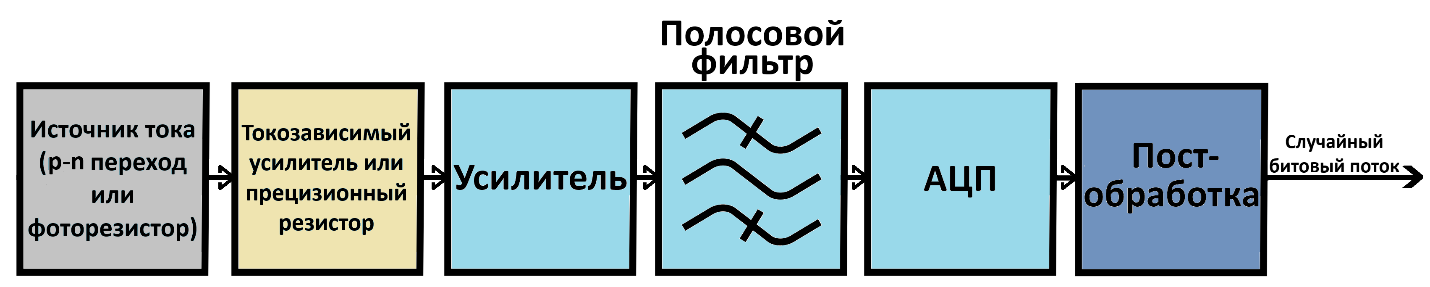
\includegraphics[width=6.49583in,height=1.30417in]{pandoc_media/media/image5.png}

Рисунок 5

\textbf{Лавинный шум} --- это разновидность дробового шума, возникающая
в полупроводниковых приборах с внутренним усилением, таких как лавинные
фотодиоды (APD, avalanche photodiodes), лавинные транзисторы,
стабилитроны или p--n переходы при пробое. Он обусловлен стохастическим
характером процесса лавинной генерации носителей, при котором один
носитель может возбуждать несколько новых носителей через ударную
ионизацию.

Когда напряжение на p--n переходе превышает определённый порог,
начинается ударная ионизация: свободные электроны, ускоряясь
электрическим полем, ионизируют атомы кристаллической решётки, создавая
новые пары электрон - дырка. Этот процесс накапливается лавинообразно и
приводит к внутреннему усилению сигнала. Поскольку число новых носителей
в каждой лавине случайно, процесс сопровождается флуктуациями, т.е.
шумом.

При учёте коэффициента внутреннего усиления M и коэффициента избыточного
шума F, спектральная плотность тока лавинного шума задаётся{[}11{]}:

\[S_{I}(f) = 2qIM^{2}F\]

где:

\begin{quote}
\(S_{I}(f)\) -- спектральная плотность тока, {[}А²/Гц{]},

\emph{q} ≈ 1,6×10\textsuperscript{−19} Кл -- заряд электрона,

\emph{I} -- средний фототок без усиления, {[}А{]},

\emph{M} -- коэффициент лавинного усиления,

\emph{F} -- коэффициент избыточного шума, зависящий от технологии
(например, \emph{F} ≈ \emph{M} при равных вероятностях ионизации
электронов и дырок).
\end{quote}

При моделировании с учётом разных ионизационных вероятностей для
электронов и дырок (k) используется приближённая формула{[}11{]}:

\[F(M) = kM + \left. \ \left( 2 - \frac{1}{M} \right.\  \right)(1 - k)\]

где: \emph{k} ∈ {[}0,1{]} -- отношение коэффициентов ионизации дырок к
электронам (для кремния \emph{k} ≪ 1, для арсенида галлия -- \emph{k} ≈
0.4).

Для построения генераторов случайных чисел на основе лавинного шума
применяются лавинные фотодиоды, работающие в режиме ниже или около
пробоя. Шум усиливается, фильтруется, оцифровывается и проходит
постобработку, как и в системах на тепловом или дробовом шуме.
Преимущество лавинного шума -- более высокая амплитуда флуктуаций, что
может повысить отношение сигнал/шум.

Преимущества:

\begin{itemize}
\item
  Очень высокий уровень шума даже при малых токах.
\item
  Возможность построения компактных источников энтропии.
\item
  Хорошо подходит для светочувствительных систем.
\end{itemize}

Недостатки:

\begin{itemize}
\item
  Сильная температурная зависимость.
\item
  Необходимость прецизионного контроля напряжения, чтобы избежать
  перехода в режим пробоя.
\item
  Лавинные процессы могут вызывать деградацию прибора со временем.
\end{itemize}

\textbf{Мерцающий шум}, также известный как шум с обратной
пропорциональностью к частоте (англ. flicker noise или \emph{1/f}
noise), представляет собой тип низкочастотного шума, который наблюдается
в широком классе электронных компонентов --- в первую очередь в
МОП-транзисторах, резисторах и других полупроводниковых приборах. Его
характерной особенностью является спектральная плотность мощности,
обратно пропорциональная частоте: \(S(f) \propto \frac{1}{f^{\gamma}}\),
где~γ ≈ 1

Физическая природа 1/f шума до конца не установлена, но в
МОП-транзисторах основной вклад в него дают следующие механизмы:

\begin{itemize}
\item
  Флуктуации числа носителей заряда (Carrier Number Fluctuation):
\end{itemize}

Происходят за счёт захвата и высвобождения носителей в ловушках на
границе оксид-полупроводник.

\begin{itemize}
\item
  Флуктуации подвижности носителей (Carrier Mobility Fluctuation):
\end{itemize}

Возникают из-за нестационарности рассеяния носителей, например, за счёт
изменения локального электрического поля.

\begin{itemize}
\item
  Комбинация CNF и CMF может приводить к коррелированным
\end{itemize}

эффектам, усиливая спектральную плотность шума

Спектральная плотность напряжения 1/f шума обычно приближённо выражается
так{[}12{]}:

\[S_{V}(f) = \frac{K}{C_{ox}^{2}WL}\frac{1}{f}\]

где:

\begin{quote}
\emph{K} --- эмпирический коэффициент, зависящий от технологического
процесса,

\(C_{ox}\) --- ёмкость оксида затвора на единицу площади,

\emph{W} и \emph{L} --- ширина и длина канала транзистора
соответственно,

\emph{f} --- частота.
\end{quote}

Таким образом, шум усиливается при уменьшении размеров транзистора,
особенно при переходе к нанометровым техпроцессам.

В сравнении с тепловым шумом, обладающем постоянной спектральной
плотностью (\(S(f) = const\)), 1/f шум, наоборот, убывает с увеличением
частоты и доминирует на низких частотах. Существует частота пересечения
(так называемая \emph{угловая частота}), выше которой 1/f шум становится
слабее теплового шума. Ниже этой частоты он начинает преобладать.

В генераторах случайных чисел (ГСЧ) 1/f шум может вызывать корреляции
между выходными битами, особенно при недостаточной скорости выборки. Это
делает его менее эффективным для генераторов, работающих на высоких
частотах. Формально, выходной сигнал ГСЧ может быть подвержен
автокорреляции:

\(Corr(X_{t},X_{t + \tau}) > 0\) при~малых~τ

где \(X_{t}\) -- выходной бит в момент времени t.

Хотя мерцающий шум сам по себе не является идеальным источником
энтропии, при правильной архитектуре он может служить источником
энтропии для низкоскоростных TRNG или добавочным источником к тепловому
или дробовому шуму.

\begin{quote}
\textbf{2.2. Оптические и квантовые источники.}
\end{quote}

Квантовая физика лежит в основе современного понимания устройства
материи. Одной из ключевых особенностей квантовых процессов является их
фундаментальная недетерминированность. Это означает, что даже при точном
знании начальных условий результат квантового измерения нельзя
предсказать однозначно. Именно это делает квантовые явления естественным
и надежным источником истинной случайности.

Классические генераторы случайных последовательностей (ГСП), в отличие
от квантовых, работают на основе детерминированных физических процессов.
Их "случайность" обусловлена только недостатком информации о начальных
параметрах системы, а потому при теоретически полной информации
поведение таких систем становится предсказуемым. В связи с этим только
квантовые ГСП можно строго научно обосновать как источники истинной
энтропии.

Квантовые генераторы случайных чисел (КГСЧ) используют одиночный
квантовый эффект, воспроизводимый в идентичных начальных условиях.
Несмотря на это, каждый эксперимент даёт непредсказуемый результат --- в
полном соответствии с законами квантовой механики.

В основе большинства КГСЧ лежит работа с кубитами --- квантовыми
аналогами битов, которые могут находиться в двух состояниях: (0) и (1),
либо в их суперпозиции. Примерами физических реализаций кубитов являются
спин электрона или поляризация фотона. При измерении кубита он «падает»
в одно из этих состояний, а результат измерения непредсказуем и
подчиняется вероятностному закону.

Система из L кубитов имеет 2\textsuperscript{L} возможных независимых
состояний. Это позволяет квантовым устройствам выполнять параллельные
вычисления и использовать квантовую суперпозицию для генерации случайных
битов.

Пример: генерация с помощью поляризованных фотонов

Часто для создания КГСЧ применяют фотоны. Их удобно создавать,
направлять и детектировать. Одна из простейших схем генерации случайных
битов заключается в пропускании фотона с круговой поляризацией через
светоделительную пластину. Она разделяет фотон на два возможных пути --
горизонтальный и вертикальный -- с равной вероятностью. Направление
выхода фотона (влево или вправо), фиксируемое соответствующим
детектором, интерпретируется как логический 0 или 1 (Рисунок 6){[}3{]}.
Даже при неизменной установке и начальных условиях результат
эксперимента каждый раз может быть разным, поскольку выбор пути фотоном
является по своей природе квантово-случайным.

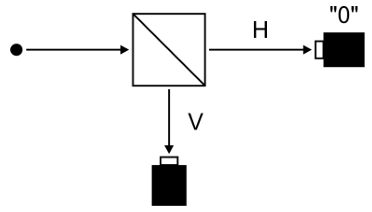
\includegraphics[width=3.87569in,height=2.20833in]{pandoc_media/media/image6.png}

Рисунок 6

Физическая случайность при использовании оптических систем основана на
фундаментально вероятностной природе некоторых квантовых процессов, в
которых фотоны участвуют. Основными механизмами получения энтропии в
оптических квантовых генераторах являются спонтанное излучение,
расщепление пучка света и измерение флуктуаций оптического поля.

Существует также подход, при котором фотонные генераторы используют
временную характеристику событий -- например, измерение интервалов между
спонтанными выбросами фотонов лазером. Такие схемы основаны на временном
принципе, противоположном пространственному, где случайность кодируется
не в месте попадания фотона, а во времени его детектирования.

В ряде решений применяется метод регистрации квантовых флуктуаций
вакуумного поля с помощью высокочувствительных детекторов, таких как
гомодинные или гетеродинные схемы. Эти системы позволяют считывать
непрерывные шумовые сигналы, содержащие истинную квантовую энтропию, и
далее оцифровывать их для получения случайных битов.

Следует отметить, что оптические схемы обладают высокой
производительностью, а некоторые современные ГИСП на основе фотонов
достигают скоростей генерации десятков гигабит в секунду. В то же время
существует ряд практических ограничений. Несмотря на высокую степень
случайности, реальная реализация КГСЧ сталкивается с рядом технических
проблем:

1. Неидеальность компонентов: расщепление пучка может быть не совсем
симметричным; детекторы могут иметь разную эффективность.

2. Старение и температурные сдвиги: с течением времени свойства
оптических и электронных компонентов могут изменяться, нарушая
равновероятность выходных состояний.

3. Корреляции между битами: вызваны, например, временем восстановления
фотонного детектора, приводят к появлению зависимостей между
результатами последовательных измерений.

Для устранения этих недостатков применяется калибровка оборудования,
схемы с одним фотонным детектором и, при необходимости, постобработка
данных, которая снижает уровень корреляций до допустимого значения.

Особое внимание уделим радиоактивному распаду в качестве источника
энтропии. Радиоактивный распад является квантовомеханическим процессом,
происходящим самопроизвольно в нестабильных атомных ядрах. Вероятность
распада за бесконечно малый промежуток времени dt описывается
экспоненциальным законом:

\(P(t) = \lambda e^{- \lambda t}\),

где:

\begin{quote}
\emph{t} -- время, прошедшее с последнего распада,

\emph{λ} -- постоянная распада, связанная с периодом полураспада
\(T_{\frac{1}{2}}\)\hspace{0pt} через отношение
\(\lambda = \frac{ln2}{T_{\frac{1}{2}}}\)
\end{quote}

Величина t носит истинно случайный характер в пределах законов квантовой
механики. Это означает, что даже при полной информации об окружающей
среде невозможно точно предсказать момент следующего распада конкретного
атома.

Таким образом, временные интервалы между последовательными актами
радиоактивного распада представляют собой случайную величину с хорошо
описанной теоретической моделью.

Типичная реализация состоит из следующих компонентов:

\begin{enumerate}
\def\labelenumi{\arabic{enumi}.}
\item
  Радиоактивный изотоп с безопасной активностью (например, америций-241
  или стронций-90).
\item
  Детектор ионизирующего излучения -- например, счётчик Гейгера-Мюллера,
  кремниевый фотодиод или сцинтиллятор.
\item
  Схема счёта времени между детекциями событий (высокоточный таймер,
  например, с частотой 1--100 МГц).
\item
  Алгоритм дискретизации времени в битовые значения.
\end{enumerate}

Пусть последовательность времён регистрации событий обозначена как
\(\{ t_{1},t_{2},\ldots,t_{n}\}\). Тогда

\[\Delta t_{i} = t_{i} - t_{i - 1}\]

представляют собой независимые и экспоненциально распределённые
величины. Эти значения могут быть использованы как вход в функцию
дискретизации, например:

\begin{quote}
Младшие k битов \(\Delta t_{i}\)\hspace{0pt} используются как случайный
битовый поток.

Или применяется функция:

\[x_{i} = \left\{ \begin{array}{r}
1,\ \ если\ \Delta t_{i} > \tau \\
0,\ \ если\ \Delta ti \leq \tau
\end{array} \right.\ \]
\end{quote}

где τ -- эмпирически выбранный порог, обеспечивающий равновероятность 0
и 1.

Для устранения возможной остаточной корреляции и аппаратных искажений
применяются криптографически стойкие экстракторы энтропии, такие как:
хэш-функции (SHA-2, BLAKE2), метод фон Неймана (Von Neumann debiasing).

Несмотря на достаточно весомое количество преимуществ такой реализации,
квантовые ГИСП на основе радиоактивного распада имеют ряд ограничений и
проблем, наиболее значительные из которых:

\begin{itemize}
\item
  Ограниченная скорость генерации (≤10\textsuperscript{4} событий в
  секунду для безопасных изотопов).
\item
  Аппаратная сложность и стоимость, включая защиту от ионизирующего
  излучения.
\item
  Юридические и нормативные ограничения на использование радиоактивных
  веществ (например, требования Росатома или IAEA).
\item
  Необходимость калибровки и тестирования детекторов, учитывая старение,
  температурную нестабильность и возможные ложные срабатывания.
\end{itemize}

\textbf{2.3. Механические и акустические источники}

Помимо квантовых и оптических методов генерации случайных чисел, в ряде
практических приложений используются механические и акустические
источники энтропии. Эти методы опираются на макроскопические процессы,
которые, несмотря на свою классическую природу, обладают высокой
чувствительностью к начальному состоянию и внешним возмущениям, что
делает их полезными в качестве дополнительных или вспомогательных
компонентов в системах генерации случайных последовательностей.

\textbf{Механические} системы используются в генераторах случайных чисел
уже десятилетия. Одним из простейших исторических примеров является
механический бросок кости или вращение рулетки. В современных
электронных системах механические элементы могут использоваться более
технологично -- например, в виде микроэлектромеханических систем (MEMS),
вибрационных датчиков или гироскопов.

Случайность в таких системах формируется за счёт хаотического характера
движения, вызванного микроскопическими флуктуациями, вибрациями,
трением, турбулентными потоками воздуха и другими стохастическими
процессами. В случае MEMS-устройств генерация энтропии может
происходить, например, при считывании отклонений подвижных элементов от
их положения равновесия.

Однако стоит учитывать, что механические источники подвержены износу,
старению, температурным деформациям, а также могут демонстрировать
ограниченный спектр случайных состояний, что требует дополнительной
обработки данных и контроля качества выходной последовательности.

\textbf{Акустические} методы используют шумы, возникающие при вибрации
объектов, прохождении звуковых волн через различные среды или при работе
механических систем. В качестве источника энтропии может применяться
электронное считывание акустического шума, например, с микрофонов или
пьезоэлектрических датчиков.

Шумы окружающей среды, звуковые помехи в помещениях, тепловые флуктуации
в материалах -- всё это создаёт уникальные и сложно моделируемые
сигналы, которые при должной обработке могут использоваться для
генерации случайных битов. Часто в таких генераторах реализуется схема с
усилением слабого акустического сигнала, его последующей оцифровкой и
выделением энтропии путём анализа амплитудных и спектральных
характеристик.

Основная особенность механических и акустических источников состоит в
том, что они относятся к классическим стохастическим системам, где
случайность возникает не из-за фундаментальной неопределённости (как в
квантовых системах), а в результате сложности и непредсказуемости
начальных условий и чувствительности к внешним воздействиям.

Поэтому такие генераторы, как правило, требуют более тщательной оценки
качества случайности, применения криптографических методов постобработки
(например, хэш-функций или выравнивающих фильтров), а также постоянного
контроля над параметрами окружающей среды.

Тем не менее, механические и акустические источники обладают весомыми
преимуществами: низкая стоимость, простота реализации, возможность
работы в условиях отсутствия других источников энтропии, а также
устойчивость к некоторым видам атак, направленным на цифровые или
оптические системы.

Примеры механических и акустических источников энтропии:

1. Гироскопические датчики и акселерометры (MEMS-ГИСП). Во многих
современных смартфонах и устройствах «умного дома» установлены
микроэлектромеханические датчики движения -- гироскопы и акселерометры.
При включении эти датчики фиксируют мельчайшие колебания, вызванные
неустранимыми шумами, механическими вибрациями корпуса, незначительными
колебаниями в условиях покоя и прочими эффектами. Эти сигналы после
усиления и оцифровки могут быть преобразованы в последовательности
случайных чисел. Некоторые реализации ГИСП в мобильных системах
используют такие датчики как резервные источники энтропии при
инициализации криптографических функций.

2. Микрофоны и пьезоэлектрические датчики акустических шумов.
Использование акустического фона помещения -- один из наиболее простых и
в то же время нестандартизируемых способов получения случайности. Шум
вентиляции, голоса, механические звуки в помещении и даже вибрации
корпуса устройства -- всё это создаёт непредсказуемую акустическую
картину. Возможно использование системы, где обычный микрофон в
помещении считывает окружающий шум, после чего аудиопоток
дискретизируется с высокой частотой, и битовая энтропия извлекается из
малозначащих битов амплитуды или частотных компонент.

3. Макроскопические механизмы (сброс шара, вращение диска). В простейших
физических ГИСП, иногда используемых в образовательных целях, случайные
события формируются на основе таких процессов, как падение шарика по
наклонной плоскости с препятствиями или вращение балансировочного диска
с многими секторами. Положение остановки или путь движения зависит от
огромного количества микрофакторов -- силы толчка, трения, мельчайших
неровностей. Система может считывать результат, например, с помощью
оптического сенсора.

4. Сейсмические датчики и вибрационные шумы. В некоторых защищённых
аппаратных платформах встраиваются сейсмодатчики, чувствительные к
микровибрациям. В условиях минимальной подвижности такие сенсоры
фиксируют флуктуации, вызванные даже шагами в соседнем помещении или
работой оборудования, преобразуя их в цифровой сигнал. Хотя это требует
высокой чувствительности, результат -- поток данных, богатый энтропией.

5. Достаточно часто, благодаря своей простоте, применяется способ сбора
энтропии из движений человеком мыши по экрану. Движение мыши -- это
результат взаимодействия множества факторов: моторика человека,
разрешение сенсора мыши, задержки ввода, скорость реакции,
нестабильность движений. Эти движения в общей массе содержат высокую
энтропию, особенно в начальные моменты, когда пользователь двигает мышь
произвольно. Примерная схема работы ГИСП на базе движения мыши может
состоять из 4 этапов:

\begin{quote}
1. Сбор координат. В фоновом режиме приложение (например, веб-страница с
JavaScript) регистрирует перемещения мыши. Координаты курсора x и y, а
также временная метка (timestamp) фиксируются в реальном времени при
каждом событии mousemove.

2. Преобразование в биты. Изменения в координатах Δx, Δy, а также
разницы времени между событиями используются для формирования числовой
последовательности. Часто берутся младшие биты (например, 1--2 младших
бита координаты или временной разницы), т.к. именно они содержат
наибольшую непредсказуемость.

3. Накопление энтропии. Пока не набрана достаточное количество битов
энтропии, генератор не начинает выдачу случайных чисел. Как правило,
ведётся оценка количества энтропии, накопленной от каждого движения
(например, 0.5 бита на каждое смещение).

4. Постобработка. После сбора достаточного количества данных

применяется хэш-функция (SHA-256, Keccak и др.), чтобы получить
финальную строку случайных битов. Это устраняет статистические
зависимости и делает вывод наиболее равномерным.
\end{quote}

\textbf{2.4. Постобработка.}

Получение последовательностей случайных битов из физических источников
энтропии, включая квантовые, тепловые, лавинные и иные генераторы, даёт
на выходе так называемые сырые данные (raw bits). Такие
последовательности не гарантируют идеального равномерного распределения
и могут содержать сдвиги, корреляции, предвзятость и другие
статистические дефекты, обусловленные воздействием окружающей среды и
вариациями технологических параметров (PVT --- process, voltage,
temperature). Поэтому требуется этап постобработки, основной задачей
которого является преобразование потока битов в статистически
выровненную и криптографически стойкую последовательность.

Постобработка (post-processing) --- это программно-аппаратный этап,
следующий за извлечением данных из физического источника. Его цель ---
удалить нежелательные закономерности, минимизировать корреляции,
устранить смещения в вероятности нуля и единицы, а также повысить
энтропию выходного потока. Формально, этот этап можно рассматривать как
применение стохастической функции:

\[f:\left\{ 0,1 \right\}^{n} \rightarrow \left\{ 0,1 \right\}^{m},m \leq n\]

где \emph{n} --- длина исходной «сырой» последовательности, \emph{m} ---
длина полученного выходного потока после фильтрации, \emph{f} ---
функция постобработки, сохраняющая энтропийную массу и стремящаяся к
равномерному распределению битов.

Существуют различные подходы к постобработке, от простых эвристик до
криптографически устойчивых трансформаций{[}3{]}{[}12{]}:

\begin{quote}
1. Специальные простые корректоры (Ad hoc Correctors):
\end{quote}

\begin{itemize}
\item
  XOR-корректоры объединяют несколько потоков из разных источников по
  операции исключающего ИЛИ:
\end{itemize}

\[b_{out} = b_{1} \oplus b_{2} \oplus \cdots \oplus b_{k}\]

где \emph{k} \textgreater{} 1 -- число независимых потоков. Метод
эффективен при независимых источниках, но снижает пропускную
способность.

\begin{itemize}
\item
  LFSR (Linear Feedback Shift Register) --- линейные регистры сдвига с
  обратной связью. Они инициализируются сырыми битами и формируют выход
  по детерминированному закону:
\end{itemize}

\[s_{i + 1} = A \cdot s_{i}\]

где \emph{A} -- матрица обратной связи. Этот метод псевдослучайный и
уязвим, если исходная энтропия мала.

\begin{itemize}
\item
  Корректор фон Неймана (von Neumann corrector, VNC) --
\end{itemize}

предназначен для устранения смещения в последовательностях случайных
битов, полученных из физических источников энтропии. Он особенно
эффективен, когда вероятности нуля и единицы на выходе не равны
\(P(0) \neq P(1)\), но предполагается, что последовательность независима
--- то есть отдельные биты не коррелированы.

Рассматриваются пары последовательных битов: \((b_{2i},b_{2i + 1})\)

Предположим, что входные биты независимы, но имеют смещение:

\begin{quote}
\[P(0) = p,P(1) = 1 - p,где\ p \neq 0.5\]
\end{quote}

Тогда вероятности появления пар:

\begin{quote}
\[P(01) = P(10) = (1 - p)p\]

\[P(00) = p^{2}\]

\[P(11) = (1 - p)^{2}\]
\end{quote}

Поэтому для каждой пары \(\left( b_{2i},b_{2i + 1} \right)\)применяется
следующее правило:

\begin{enumerate}
\def\labelenumi{\arabic{enumi}.}
\item
  Если пара равна (0,1), то на выход подаётся бит 1
\item
  Если пара равна (1,0), то на выход подаётся бит 0
\item
  Если пара равна (0,0) или (1,1), пара отбрасывается
\end{enumerate}

Таким образом появления 0 и 1 в выходном битовом потоке приобретают
равную вероятность.

2. «Отбеливание» (whitening) последовательностей с помощью
криптографических хэш-функций. Одной из самых известных техник
постобработки является «отбеливание» выходных данных генератора истинно
случайных чисел с помощью криптографической хэш-функции. Наиболее
известными являются такие хэш-функции, как MD5, SHA-1, SHA-2, SHA-256,
SHA-512. Считается, что если имеющие недостатки выходные
последовательности генератора случайных чисел пропустить через
хэш-функцию, то их качество значительно улучшится. На самом деле
показано, что хэширование «плохого» генератора может не повысить
случайность до уровня, достаточного для прохождения статистических
тестов

3. Экстрактор случайности -- это алгоритм, который преобразует длинную
слабо случайную последовательность в более короткую последовательность,
обладающую почти идеальной случайностью. Экстракторы реализуют
теоретико-информационные трансформации, приближающие выход к
равномерному распределению даже при наличии неидеальных входных данных.
Они часто строятся на основе линейных или полиномиальных преобразований.
Проблемой таких алгоритмов является то, что для их работы необходим
буфер памяти, а также мощный процессор, что замедляет скорость выходного
потока битов.

4. Упругие функции. Еще один подход к усилению случайности путем
фильтрации через некоторый детерминированный процесс -- это
использование упругих функций, которые были введены Сунаром, Мартином и
Стинсоном в качестве шага постобработки для ГСП на свободных
осцилляторах. Это логические схемы, сохраняющие случайность на выходе
даже при частичной компрометации входа. Пример: мажоритарная логика,
блоки совмещённых множественных входов.

Постобработка может быть реализована:

\begin{itemize}
\item
  Аппаратно (on-chip): для простых корректоров и базового whitening.
\item
  Программно (off-chip): для хэшей, криптографических функций,
  экстракторов.
\end{itemize}

Постобработка является неотъемлемым этапом в архитектуре генераторов
истинно случайных чисел. От качества её реализации зависит не только
статистическая полнота выходной последовательности, но и её пригодность
для криптографических и стохастических приложений. Правильный выбор
алгоритма зависит от компромисса между пропускной способностью,
аппаратной сложностью и требуемым уровнем безопасности. Однако даже
идеальная постобработка не может компенсировать слабость или атакуемость
физического источника. Как подчёркивает стандарт NIST SP 800-90A, для
использования в криптографических целях требуется:

\begin{itemize}
\item
  Наличие процедуры тестирования источника на месте (health testing),
\item
  Использование стойкой к атакам постобработки,
\item
  Оценка энтропии на входе.
\end{itemize}

\textbf{2.5. Уязвимости и атаки.}

Оценка устойчивости генераторов истинной случайности является
неотъемлемой частью обеспечения криптографической безопасности. В
прикладной криптографии принято анализировать уязвимости каждого
компонента системы в отдельности, поскольку компрометация даже одного
элемента может поставить под угрозу всю систему. В частности, ГИСП, как
источник энтропии, представляет особый интерес, поскольку его выход
должен быть максимально непредсказуем.

Атаки на ГИСП подразделяются на две большие группы -- пассивные и
активные. Пассивные атаки направлены на получение информации о
внутреннем состоянии генератора без физического вмешательства в его
работу. Цель таких атак -- предсказать будущие значения генератора с
ненулевой вероятностью. Активные атаки, напротив, предполагают
вмешательство в функционирование ГИСП с целью контролировать его
поведение или исказить выходные данные. Возвращаясь к модульному
представлению общей структуры ГИСП, рассмотрим рисунок 7{[}12{]}:

\begin{figure}
\centering
\pandocbounded{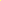
\includegraphics[keepaspectratio]{pandoc_media/media/image7.png}}
\caption{}
\end{figure}

\begin{figure}
\centering
\pandocbounded{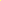
\includegraphics[keepaspectratio]{pandoc_media/media/image7.png}}
\caption{1}
\end{figure}

\begin{figure}
\centering
\pandocbounded{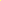
\includegraphics[keepaspectratio]{pandoc_media/media/image7.png}}
\caption{2}
\end{figure}

\begin{figure}
\centering
\pandocbounded{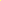
\includegraphics[keepaspectratio]{pandoc_media/media/image7.png}}
\caption{3}
\end{figure}

\begin{figure}
\centering
\pandocbounded{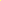
\includegraphics[keepaspectratio]{pandoc_media/media/image7.png}}
\caption{4}
\end{figure}

\begin{figure}
\centering
\pandocbounded{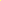
\includegraphics[keepaspectratio]{pandoc_media/media/image7.png}}
\caption{4}
\end{figure}

\begin{figure}
\centering
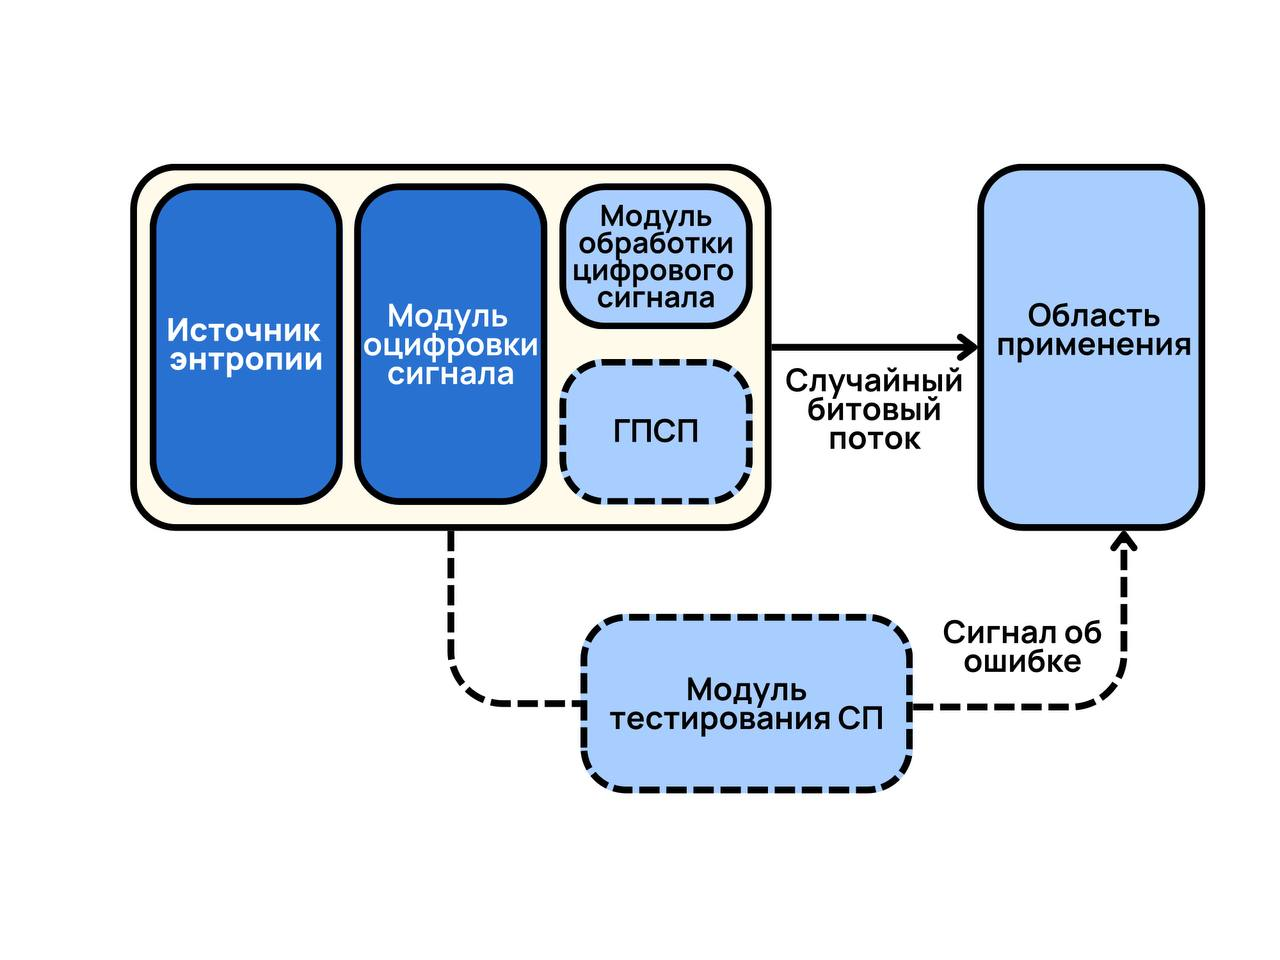
\includegraphics[width=4.68611in,height=2.89514in]{pandoc_media/media/image1.png}
\caption{5}
\end{figure}

Рисунок 7

Возможными направлениями для пассивных атак будут: 1, 5. Для активных --
1, 2, 3, 4.

Одним из наиболее изученных классов атак являются атаки через побочные
каналы (SCA, side-channel attacks). Эти методы используют измерения
физических параметров устройства, таких как потребляемая мощность,
электромагнитное излучение, временные задержки или звуковые колебания.
Например, в случае генераторов на основе кольцевых осцилляторов (RO)
было показано, что они уязвимы к активным электромагнитным атакам. При
помощи дифференциального частотного анализа исследователям удалось
извлечь информацию о частотах и расположении осцилляторов. Это, в свою
очередь, позволило провести точную синхронизацию осцилляторов, что
разрушает источник энтропии (джиттер) и делает выход ГИСП предсказуемым.

Другой тип атак -- инъекция ошибок (fault injection) -- предполагает
преднамеренное внесение сбоев в работу схемы. Для этого могут
использоваться такие внешние воздействия, как высокие или экстремально
низкие температуры, мощные электромагнитные поля или интенсивное
освещение. Особенно уязвимы ГИСП на базе свободно работающих
осцилляторов: например, если в питающую цепь подать внешнюю частоту,
можно зафиксировать фазу осцилляции, устранив случайность в выходном
сигнале (Рисунок 8){[}14{]}.

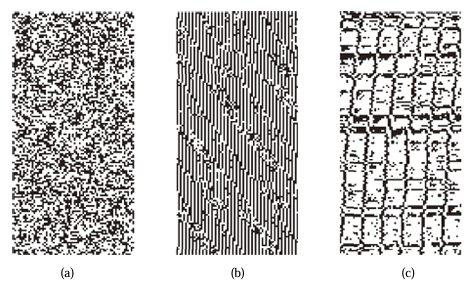
\includegraphics[width=4.93819in,height=3.00069in]{pandoc_media/media/image8.png}

Рисунок 8.

Атака с использованием частотной инъекции

(a) исходный битовый поток ГИСП (70*140)

(b) инъекция с частотой 1,822880 МГц

(c) инъекция с частотой 1,929629 МГц

Современные достижения в области машинного обучения открыли возможности
для интеллектуальных атак на ГИСП. Одно из исследований
продемонстрировало, что, модифицируя битстрим FPGA-реализации ГИСП
(добавляя сотни дополнительных триггеров), можно обучить модель
глубокого обучения распознавать шаблоны в распределении потребляемой
мощности. Хотя такая атака требует внедрения стороннего кода и потому не
считается полной компрометацией, она подчёркивает потенциальную
опасность аппаратных троянов и направленных ML-атак в будущем.

Для защиты от подобных угроз предлагается несколько мер. Во-первых,
важно физически изолировать чувствительные компоненты ГИСП, например,
размещать развязывающие конденсаторы рядом с кольцевыми осцилляторами.
Во-вторых, структура самого ГИСП должна быть оптимизирована для
устойчивости к внешним воздействиям. Наконец, критически важно внедрение
онлайн-механизмов самотестирования, способных в реальном времени
отслеживать и сигнализировать о любых аномалиях в поведении генератора.

Таким образом, надёжность ГИСП определяется не только качеством
источника энтропии, но и устойчивостью ко множеству атак. Это требует
системного подхода к проектированию и постоянного контроля за состоянием
генератора в процессе эксплуатации.

\textbf{\hfill\break
}

\textbf{ГЛАВА 3. Сравнительная характеристика и перспективы применения}

\textbf{3.1. Сравнительный анализ источников энтропии}

Сравнение различных физических и квантовых источников энтропии
показывает, что каждый из них обладает уникальными преимуществами и
ограничениями, что делает их пригодными для разных сфер применения в
зависимости от конкретных требований к качеству случайности, уровню
безопасности, потребляемым ресурсам и технологическим возможностям
интеграции.

Физические источники энтропии, такие как тепловой шум, дробовой шум,
лавинный шум и мерцающий шум, характеризуются относительно простой
схемотехнической реализацией и возможностью интеграции в существующие
полупроводниковые платформы. Это делает их особенно привлекательными для
встраивания в микроконтроллеры, криптографические процессоры и другие
устройства массового производства. Однако такие источники могут быть
чувствительны к температурным колебаниям, электромагнитным наводкам,
старению компонентов и другим нежелательным факторам, которые могут
вносить детерминированные искажении в сигнал, снижая истинную энтропию.
Например, тепловой шум достаточно стабилен, но имеет сравнительно низкую
энтропийную мощность, что ограничивает его скорость генерации. Дробовой
и лавинный шумы более насыщены энтропией и менее предсказуемы, но
требуют сложной схемы усиления и фильтрации, а также могут генерировать
импульсные сигналы, неравномерные по амплитуде и длительности. Мерцающий
шум отличается высокой интенсивностью при низких частотах, но сложен для
оценки и контроля, а также может быть подвержен воздействию окружающей
среды.

Квантовые источники энтропии, основанные на таких явлениях, как
квантовые переходы, туннелирование, спонтанное излучение или рассеяние
фотонов, обеспечивают наивысший уровень истинной случайности, поскольку
происхождение сигнала невозможно описать детерминированными законами
физики. Это делает такие источники предпочтительными для задач, где
требуется абсолютная непредсказуемость, например, в генерации ключей для
квантово-устойчивой криптографии. Однако их реализация требует
прецизионной оптики, фотонных детекторов, лазеров или других сложных
квантово-оптических компонентов. Это не только увеличивает стоимость
устройств, но и требует особых условий эксплуатации, включая защиту от
вибраций, температурную стабилизацию и экранирование от внешних
воздействий. Кроме того, из-за высокой чувствительности к шумам и дрейфу
параметров оборудования, такие системы нуждаются в регулярной калибровке
и контроле качества работы.

Макроскопические и хаотические источники энтропии основаны на трудно
моделируемых динамических процессах, таких как движение в турбулентных
потоках, случайные колебания в нелинейных цепях или шум в радиоэфире.
Они интересны прежде всего своей простотой в реализации и возможностью
достигать очень высокой скорости генерации, что особенно полезно для
приложений, не связанных с криптографией, но требующих большого
количества случайных данных (например, в компьютерных играх или
симуляционных моделях). Однако эти источники страдают от высокой
зависимости от внешних условий и трудно поддаются строгой математической
верификации, что делает их менее надёжными в задачах, где требуется
доказуемо высокая энтропия. Кроме того, при известной модели системы, в
теории, возможно частичное предсказание поведения хаотического
источника, особенно если используется псевдослучайный усилитель
динамики.

В обобщении, можно сказать, что физические источники -- это компромисс
между простотой, скоростью и надёжностью, квантовые -- максимум
безопасности и непредсказуемости при высокой стоимости, а хаотические --
высокая производительность при умеренном уровне доверия. Поэтому выбор
зависит от того, что критично в конкретной системе: высокая скорость,
минимальные затраты, интегрируемость или гарантированная случайность.

\textbf{3.2. Перспективные направления развития физических генераторов
случайных последовательностей (ФГСП)}

Современные требования к безопасности информационных систем, а также
рост применения криптографических и статистических методов в различных
областях обуславливают необходимость дальнейшего совершенствования
физических генераторов случайных последовательностей (ФГСП). Развитие
данных систем направлено на повышение их надёжности, устойчивости к
внешним воздействиям, скорости генерации и интеграции в современные
аппаратные платформы. Ниже рассмотрены ключевые направления развития.

Миниатюризация и интеграция в чипы. Современные технологии производства
микросхем позволяют встраивать элементы ФГСП непосредственно в
процессоры, контроллеры и криптографические сопроцессоры. Это
обеспечивает минимальные задержки при получении случайных битов и
упрощает защиту от атак на уровне интерфейсов. Развитие технологии CMOS,
FinFET и перспективных материалов способствует созданию компактных,
энергоэффективных и массовых решений.

Перспективным направлением является использование квантовых источников
энтропии -- в частности, спонтанного распада фотонов, квантовых
флуктуаций вакуума и эффекта туннелирования. Такие источники обладают
высокой степенью истинной случайности, подтверждаемой теорией квантовой
неопределённости, и демонстрируют устойчивость к предсказуемости со
стороны атакующего. Разработка доступных и стабильно работающих
квантовых ФГСП, увеличение скорости их генерации остаются важной
задачей.

Оптические и фотонные источники также могут быть подвержены
модернизации. Оптические ФГСП, основанные на фотоэлектрическом шуме,
колебаниях интенсивности лазерного излучения и спонтанном рассеянии
света, демонстрируют высокую пропускную способность и низкую
коррелированность выходных битов. Развитие интегральной фотоники и
кремниевых фотонных чипов позволяет создавать компактные и
масштабируемые оптические генераторы с высокой скоростью и надёжностью.

Повышение надёжности генерации достигается за счёт объединения
нескольких физических источников энтропии в гибридной архитектуре.
Комбинация теплового, дробового, лавинного шумов, а также оптических и
квантовых источников позволяет компенсировать слабости отдельных
компонентов, а также реализовать адаптивные схемы оценки качества и
селекции наиболее надёжных источников в реальном времени. Таким образом,
перспективным направлением развития является изучение комбинаций
источников энтропии в ФГСП: многоканальные и гибридные схемы.

Совершенствование методов постобработки, внедрение постобработки на
аппаратном уровне также являются современной тенденцией развития ФГСП.
Для повышения энтропийной насыщенности и устранения смещения (bias)
усиливается внимание к аппаратной реализации алгоритмов экстракции,
таких как схема фон Неймана, хэш-функции и решёточные методы. Аппаратная
реализация постобработки позволяет достичь высокой скорости и
энергоэффективности без ущерба для статистических свойств выходных
данных.

Современные подходы к верификации и мониторингу работы ФГСП
предусматривают встраивание модулей контроля, способных выполнять
непрерывное статистическое тестирование и выявление деградации качества
энтропии. Это особенно важно в критических приложениях, где отклонения в
характеристиках могут привести к серьёзным уязвимостям. С появлением
новых способов атаки на ФГСП также появляется необходимость в
поддержании эффективного автоматического тестирования и самодиагностики.

В рамках международных инициатив (например, NIST, ISO) разрабатываются
единые подходы к оценке качества ФГСП. Это способствует унификации
требований, повышению доверия к устройствам и упрощению их внедрения в
сертифицированные системы безопасности.

В совокупности данные направления определяют вектор дальнейших
исследований и разработок в области ФГСП, ориентируясь на создание
высоконадёжных, воспроизводимых и проверяемых источников истинной
случайности для современных и перспективных информационно-технических
систем.

\textbf{ЗАКЛЮЧЕНИЕ}

В рамках данной курсовой работы была проведена комплексная оценка
физических генераторов случайных последовательностей (ФГСП), основанных
на различных источниках энтропии. Изучение теоретических основ позволило
выделить важные свойства случайных чисел, отличать истинную случайность
от псевдослучайности, а также понять роль энтропии как ключевого ресурса
в криптографических и инженерных системах. Особое внимание было уделено
методам статистической проверки качества случайных последовательностей,
включая тесты частоты, последовательности бит, оценки энтропии и другие
критерии из NIST STS.

Во второй главе были подробно рассмотрены физические источники энтропии,
применяемые в аппаратных ГСП. Электронные источники включали тепловой,
лавинный, дробовой и мерцающий шумы. Для каждого из них рассмотрены
принципы генерации, аппаратная реализация, устойчивость к внешним
факторам и особенности практического применения. Установлено, что такие
источники, как лавинный и дробовой шум, позволяют реализовывать
компактные и сравнительно простые устройства, однако при этом требуют
учета технических ограничений, таких как чувствительность к температуре
или необходимость в усилении сигнала. Тепловой шум обеспечивает хорошую
воспроизводимость и низкую стоимость, в то время как мерцающий шум слабо
пригоден к использованию из-за сложности выделения полезного сигнала.

Оптические и квантовые источники, описанные во второй части главы,
открывают перспективы для создания генераторов с высокой энтропийной
мощностью и принципиально непредсказуемым поведением. Их реализация, как
правило, требует сложной оптоэлектронной аппаратуры, но зато
обеспечивает высокую теоретическую безопасность и потенциальную
устойчивость к широкому классу атак. Отдельно отмечены возможности
использования эффектов квантовой интерференции, туннелирования и
спонтанной эмиссии фотонов в качестве надёжных первоисточников
случайности.

Анализ механических и акустических источников показал, что, несмотря на
их простоту и низкую стоимость, данные методы обладают низкой
стабильностью, значительной зависимостью от внешней среды и невысокой
скоростью генерации. Однако в специфических условиях (например, в
автономных системах или устройствах сбора случайных данных из окружающей
среды) такие источники могут найти применение.

Глава, посвящённая постобработке, подчеркнула важность цифровой
обработки для повышения качества получаемых последовательностей.
Указано, что даже физически случайные сигналы могут содержать
коррелированные участки, требующие использования хеш-функций,
декоррелирующих фильтров и нормализаторов. Методы оценки и устранения
ошибок критически важны при внедрении ФГСП в ответственных
криптографических системах.

Сравнительный анализ, представленный в третьей главе, обобщил полученные
данные, выделив достоинства и недостатки каждого типа источников. По
совокупности характеристик наилучшие показатели стабильности и скорости
продемонстрировали лавинные и квантовые генераторы. В то же время
дробовой шум оказался сбалансированным решением по совокупности
критериев: надёжности, простоты реализации и чувствительности к внешним
воздействиям. Также была обозначена высокая чувствительность некоторых
источников к помехам, что требует проведения экранирования или
компенсации шумов при проектировании.

Наконец, в разделе о перспективах развития рассмотрены технологические и
теоретические направления, способные повлиять на развитие аппаратных
генераторов в ближайшие годы: это миниатюризация компонентов, внедрение
в стандартные микросхемы, повышение энергоэффективности и
самотестируемости, а также дальнейшее развитие квантовых источников как
наиболее надёжной формы получения энтропии.

Таким образом, проведённое исследование подтвердило актуальность и
сложность выбора подходящего источника энтропии для проектирования
надёжных аппаратных генераторов. Полученные результаты могут служить
основой для разработки и оптимизации ФГСП, адаптированных под конкретные
задачи в области информационной безопасности, криптографии и инженерных
систем.

\textbf{СПИСОК ИСПОЛЬЗОВАННЫХ ИСТОЧНИКОВ}

\begin{enumerate}
\def\labelenumi{\arabic{enumi}.}
\item
  Android Security Vulnerability {[}URL{]}:
\end{enumerate}

\url{https://bitcoin.org/en/alert/2013-08-11-android}

\begin{enumerate}
\def\labelenumi{\arabic{enumi}.}
\setcounter{enumi}{1}
\item
  Матвеев Ю.Н. Цифровая обработка сигналов {[}Текст{]}: учебное
\end{enumerate}

пособие / Матвеев Ю.Н., Симончик К.К., Тропченко А.Ю., Хитров М.В. --
СПб: СПбНИУ ИТМО, 2013. -- 166 с.

\begin{enumerate}
\def\labelenumi{\arabic{enumi}.}
\setcounter{enumi}{2}
\item
  Будько, М.Б. Методы генерации и тестирования случайных
\end{enumerate}

последовательностей {[}Текст{]}: учебное пособие / М.Б. Будько, М.Ю.
Будько, А.В. Гирик, В.А. Грозов. -- Санкт-Петербург: Университет ИТМО,
2019. -- 112 с.

\begin{enumerate}
\def\labelenumi{\arabic{enumi}.}
\setcounter{enumi}{3}
\item
  Слеповичев, И.И. Генераторы псевдослучайных чисел {[}Текст{]}:
\end{enumerate}

учебное пособие / И.И. Слеповичев. -- Саратовский государственный
университет, 2017. -- 118 с.

\begin{enumerate}
\def\labelenumi{\arabic{enumi}.}
\setcounter{enumi}{4}
\item
  Barker E. A Statistical Test Suite for Random and Pseudorandom
\end{enumerate}

Number Generators for Cryptographic Applications. {[}Текст{]}. / Rukhin
A., Soto J., Nechvatal J., Smid M., Leigh S., Levenson M., Vangel M.,
Banks D., Heckert A., Dray J., Vo S. -- Gaithersburg: NIST, 2010. --
131с.

\begin{enumerate}
\def\labelenumi{\arabic{enumi}.}
\setcounter{enumi}{5}
\item
  Di Mauro J., Salazar E., Scolnik H.D. Design and Implementation of a
\end{enumerate}

Novel Cryptographically Secure Pseudorandom Number Generator
{[}Текст{]}. / Di Mauro J., Salazar E., Scolnik H.D. -- Journal of
Cryptographic Engineering, 2022. -- 23 с.

\begin{enumerate}
\def\labelenumi{\arabic{enumi}.}
\setcounter{enumi}{6}
\item
  Архангельская, А.В. Построение высокоскоростных квантовых
\end{enumerate}

генераторов случайных чисел для систем защиты информации {[}Текст{]}. /
А.В. Архангельская. -- Санкт-Петербург, 2008. -- 182 с.

\begin{enumerate}
\def\labelenumi{\arabic{enumi}.}
\setcounter{enumi}{7}
\item
  Гриненко, Т.А. Статистическое тестирование генераторов
\end{enumerate}

случайных и псевдослучайных чисел с использованием набора статистических
тестов NIST STS {[}Текст{]}: учебное пособие / Т.А. Гриненко, А.В.
Потий, С.Ю. Орлова -- Харьковский государственный технический
университет радиоэлектроники, 2019. -- № 1. -- 73 с.

\begin{enumerate}
\def\labelenumi{\arabic{enumi}.}
\setcounter{enumi}{8}
\item
  Петров, Д.О. Диоды как источник энтропии для аппаратных
\end{enumerate}

генераторов случайных чисел {[}Текст{]}. / Д.О. Петров, В.В. Буслюк,
С.С. Дереченник, В.А. Емельянов -- Брестский государственный технический
университет. Серия: Радиоэлектроника и связь, 2020. -- № 4. -- 149 с.

\begin{enumerate}
\def\labelenumi{\arabic{enumi}.}
\setcounter{enumi}{9}
\item
  Григорьев, А.Ю. Методы тестирования генераторов случайных и
\end{enumerate}

псевдослучайных последовательностей {[}Текст{]}: ученые записки / А.Ю.
Григорьев - УлГУ. Сер. Математика и информационные технологии, -- 2017.
-- № 1. -- 8 с.

\begin{enumerate}
\def\labelenumi{\arabic{enumi}.}
\setcounter{enumi}{10}
\item
  Якимов, А.В. Физика шумов и флуктуаций параметров {[}Текст{]}:
\end{enumerate}

электронное учебное пособие / А.В. Якимов -- Нижегородский
госуниверситет, 2013. -- 85 с.

\begin{enumerate}
\def\labelenumi{\arabic{enumi}.}
\setcounter{enumi}{11}
\item
  Cao Y. Entropy Sources Based on Silicon Chips: True Random Number
\end{enumerate}

Generator and Physical Unclonable Function {[}Текст{]}. / Cao Y., Liu
W., Qin L., Liu B., Chen S., Ye J., Xia X., Wang C. -- Entropy, -- 2022.
-- Vol. 24(2). -- Article 241.

\begin{enumerate}
\def\labelenumi{\arabic{enumi}.}
\setcounter{enumi}{12}
\item
  Алейник, А.С. Основы схемотехники приемопередающих
\end{enumerate}

электронных устройств {[}Текст{]}: учебно-методическое пособие / А.С.
Алейник, Е.В. Востриков, С.А. Волковский, И.Г. Дейнека, В.Е. Стригалев,
И.К. Мешковский -- Санкт-Петербург: Университет ИТМО, 2021. -- 151 с.

\begin{enumerate}
\def\labelenumi{\arabic{enumi}.}
\setcounter{enumi}{13}
\item
  Markettos T., The Frequency Injection Attack on Ring-Oscillator-Based
\end{enumerate}

True Random Number Generators // CHES 2009: Cryptographic Hardware and
Embedded Systems {[}Текст{]}: Lecture Notes in Computer Science, vol
5747 / Markettos T., Moore S.W. -- Springer, 2009. -- 16 с.

\textbf{\hfill\break
}

\textbf{ПРИЛОЖЕНИЕ 1 -- Статистические тесты пакета NIST STS}

{\def\LTcaptype{none} % do not increment counter
\begin{longtable}[]{@{}
  >{\raggedright\arraybackslash}p{(\linewidth - 4\tabcolsep) * \real{0.0493}}
  >{\raggedright\arraybackslash}p{(\linewidth - 4\tabcolsep) * \real{0.3377}}
  >{\raggedright\arraybackslash}p{(\linewidth - 4\tabcolsep) * \real{0.6027}}@{}}
\toprule\noalign{}
\begin{minipage}[b]{\linewidth}\raggedright
№
\end{minipage} & \begin{minipage}[b]{\linewidth}\raggedright
Статистический тест
\end{minipage} & \begin{minipage}[b]{\linewidth}\raggedright
Описание теста
\end{minipage} \\
\midrule\noalign{}
\endhead
\bottomrule\noalign{}
\endlastfoot
1 & Частотный побитовый тест (Frequency Test) & Проверяет баланс между
количеством нулей и единиц в последовательности. Ожидается, что в
достаточно длинной случайной последовательности их соотношение будет
близко к 1:1. \\
2 & Частотный блочный тест (Frequency Test within a Block) & Частотный
побитовый тест, проводимый в отдельных блоках фиксированного размера \\
3 & Тест на последовательность одинаковых бит (Runs Test) & Анализирует
чередование нулей и единиц. Проверяет, нет ли слишком длинных серий
подряд идущих одинаковых битов. \\
4 & Тест на совпадение неперекрывающихся шаблонов (Non-overlapping
Template Matching Test) & Ищет заданные шаблоны в последовательности.
Цель --- выявить ГСП (ГПСП), формирующие слишком часто заданные
непериодические шаблоны \\
5 & Тест на периодичность (Serial Test) & Данный тест заключается в
подсчете частоты всех возможных перекрываний шаблонов длины~\emph{m}~бит
на протяжении исходной последовательности битов. Целью является
определение действительно ли количество появлений
2\emph{\textsuperscript{m}}~перекрывающихся шаблонов
длиной~\emph{m}~бит, приблизительно такое же как в случае абсолютно
случайной входной последовательности бит. Последняя, как известно,
обладает однообразностью, то есть каждый шаблон длиной~\emph{m}~бит
появляется в последовательности с одинаковой вероятностью. Если
вычисленное в ходе теста значение вероятности~\emph{p}~\textless{} 0,01,
то данная двоичная последовательность не является абсолютно
случайной. \\
6 & Тест рангов бинарных матриц (Binary Matrix Rank Test) & Разбивает
последовательность на матрицы и вычисляет их ранг. Случайные данные
должны давать ранг, близкий к теоретически ожидаемому. \\
7 & Тест приблизительной энтропии (Approximate Entropy Test) & Как и
в~тесте на периодичность~в данном тесте акцент делается на подсчёте
частоты всех возможных перекрываний шаблонов длины~\emph{m}~бит на
протяжении исходной последовательности битов. Цель теста --- сравнить
частоты перекрывания двух последовательных блоков исходной
последовательности с длинами~\emph{m}~и~\emph{m+1}~с частотами
перекрывания аналогичных блоков в абсолютно случайной
последовательности. Вычисляемое в ходе теста значение
вероятности~\emph{p}~должно быть не меньше 0,01. В противном случае
(\emph{p}~\textless{} 0,01), двоичная последовательность не является
абсолютно случайной. \\
8 & Тест кумулятивных сумм (Cumulative Sums Test) & Тест заключается в
максимальном отклонении (от нуля) при произвольном обходе, определяемым
кумулятивной суммой заданных (-1, +1) цифр в последовательности. Цель
данного теста --- определить является ли кумулятивная сумма частичных
последовательностей, возникающих во входной последовательности, слишком
большой или слишком маленькой по сравнению с ожидаемым поведением такой
суммы для абсолютно случайной входной последовательности. \\
9 & Тест на самую длинную последовательность «1» в блоке (Longest Run of
Ones Test) & Определяет максимальную длину серии единиц в блоках
фиксированного размера. \\
10 & Тест на совпадение перекрывающихся шаблонов (Overlapping Template
Matching Test) & Аналогичен тесту 4, но шаблоны могут перекрываться.
Полезен для выявления скрытых периодичностей. \\
11 & Тест на линейную сложность (Linear Complexity Test) & Оценивает,
насколько сложно воспроизвести последовательность с помощью линейного
регистра сдвига. Высокая сложность --- признак хорошей случайности. \\
12 & Спектральный тест (Discrete Fourier Transform Test) & Преобразует
последовательность в частотную область и ищет пики, которые могут
указывать на периодичность. \\
13 & Универсальный статистический тест Маурера (Maurer Universal Test) &
Измеряет "сжимаемость" последовательности. Случайные данные не должны
быть алгоритмически сжимаемы. \\
14 & Тест на произвольные проходы (Random Excursions Test) & Анализирует
случайные блуждания, построенные на основе последовательности.
Проверяет, соответствуют ли они теоретическому распределению. \\
15 & Тест на произвольные проходы (вариант) (Random Excursions Variant
Test) & Дополняет тест 14, исследуя конкретные состояния блужданий. \\
\end{longtable}
}

\textbf{ПРИЛОЖЕНИЕ 2 -- Сравнительная таблица характеристик источников
энтропии}

{\def\LTcaptype{none} % do not increment counter
\begin{longtable}[]{@{}
  >{\raggedright\arraybackslash}p{(\linewidth - 14\tabcolsep) * \real{0.1251}}
  >{\raggedright\arraybackslash}p{(\linewidth - 14\tabcolsep) * \real{0.1251}}
  >{\raggedright\arraybackslash}p{(\linewidth - 14\tabcolsep) * \real{0.1020}}
  >{\raggedright\arraybackslash}p{(\linewidth - 14\tabcolsep) * \real{0.0888}}
  >{\raggedright\arraybackslash}p{(\linewidth - 14\tabcolsep) * \real{0.1186}}
  >{\raggedright\arraybackslash}p{(\linewidth - 14\tabcolsep) * \real{0.1629}}
  >{\raggedright\arraybackslash}p{(\linewidth - 14\tabcolsep) * \real{0.0889}}
  >{\raggedright\arraybackslash}p{(\linewidth - 14\tabcolsep) * \real{0.1887}}@{}}
\toprule\noalign{}
\begin{minipage}[b]{\linewidth}\raggedright
\textbf{Источник}
\end{minipage} & \begin{minipage}[b]{\linewidth}\raggedright
\textbf{Спектральный тип шума}
\end{minipage} & \begin{minipage}[b]{\linewidth}\raggedright
\textbf{Скорость генерации}
\end{minipage} & \begin{minipage}[b]{\linewidth}\raggedright
\textbf{Качество энтропии}
\end{minipage} & \begin{minipage}[b]{\linewidth}\raggedright
\textbf{Сложность реализации}
\end{minipage} & \begin{minipage}[b]{\linewidth}\raggedright
\textbf{Устойчивость к внешним воздействиям}
\end{minipage} & \begin{minipage}[b]{\linewidth}\raggedright
\textbf{Защита от атак/моделирования}
\end{minipage} & \begin{minipage}[b]{\linewidth}\raggedright
\textbf{Комментарии / Примеры применения}
\end{minipage} \\
\midrule\noalign{}
\endhead
\bottomrule\noalign{}
\endlastfoot
\textbf{Тепловой шум} & \multirow{2}{=}{Белый шум} & Средняя
(\textasciitilde10⁴--10⁶ бит/с) & Среднее & Низкая & Средняя (зависит от
сопротивления, температуры) & Низкая--средняя & Часто используется в
IC-TRNG, требует постобработки \\
\textbf{Дробовой шум} & & Средняя--высокая & Среднее-высокое & Средняя &
Средняя--высокая (дискретность тока более устойчива) & Средняя & Широко
применяется в простых TRNG (на туннельных диодах) \\
\textbf{Лавинный шум} & Широкополосный с пиками & Высокая
(\textasciitilde10⁶--10⁸ бит/с) & Высокое & Средняя--высокая &
Средняя--высокая (зависит от порога пробоя) & Средняя- высокая &
Популярен в лавинных фотодиодах, хорош для встроенных TRNG \\
\textbf{Мерцающий шум (1/f)} & Розовый шум & Низкая (\textless10³ бит/с)
& Низкое & Низкая & Низкая (параметры сильно "плавают", нестабильность
спектра) & Низкая & Подвержен внешнему влиянию, требует усиленной
фильтрации \\
\textbf{Квантово-оптический (фотонный делитель)} & \multirow{2}{=}{Белый
(дискретные события)} & Очень высокая (\textasciitilde10⁶--10⁹ бит/с) &
Очень высокое & Высокая & Высокая (если стабилизирован лазер, фотонный
канал, питание) & Очень высокая & QRNG, QKD, сертифицированные квантовые
генераторы \\
\textbf{Радиоактивный распад} & & Очень низкая (\textasciitilde1--10³
бит/с) & Очень высокое & Очень

высокая & Очень

высокая (независим от внешней среды) & Очень высокая & Эталонные ГИСП,
используются в высокозащищённых системах \\
\textbf{Механический источник} & \multirow{2}{=}{Спектр зависит от
конфигурации (часто псевдобелый)} & Низкая (\textless10² бит/с) & Низкое
& Низкая & \multirow{2}{=}{Низкая

(вибрации, шумы подвержены массе факторов)} & Очень низкая &
Демонстрационные устройства, устаревшие игровые автоматы \\
\textbf{Акустический источник} & & Низкая & Низкое & Низкая & & Очень
низкая & Вспомогательная энтропия для ОС (например, Linux entropy
pool) \\
\end{longtable}
}

Пояснение.

Качество энтропии:

\begin{itemize}
\item
  Низкое -- сильно коррелированные значения, шум подвержен дрейфу,
  требуется мощная постобработка,
\item
  Среднее -- частично предсказуемые биты, возможен bias, возможна
  частичная корреляция,
\item
  Высокое -- почти идеальная равномерность и непредсказуемость, даже до
  постобработки.
\end{itemize}

Защита от атак/моделирования:

\begin{itemize}
\item
  Низкая -- источник уязвим к подделке, легко смоделировать или
  заглушить.
\item
  Средняя -- требуется физический доступ или точная настройка атаки
\item
  Высокая -- крайне сложно предсказать, атака невозможна без
  вмешательства в систему
\end{itemize}

\end{document}
